
\documentclass[10pt,conference,letterpaper]{IEEEtran}
\usepackage{times,amsmath,epsfig}
%\usepackage{algorithm}
\usepackage{algorithmic}
\usepackage[linesnumbered,boxed,ruled,commentsnumbered]{algorithm2e}
\usepackage{epstopdf}
\usepackage{graphicx}
\renewcommand{\algorithmicrequire}{\textbf{Input:}}
\renewcommand{\algorithmicensure}{\textbf{Output:}}
\usepackage[tight,footnotesize]{subfigure}
\usepackage{amsfonts}
\usepackage{xspace}
\usepackage{bbm}
%\usepackage{balance}


\newcommand{\tabincell}[2]{\begin{tabular}{@{}#1@{}}#2\end{tabular}}
\newcommand{\frname}{GAT\xspace }
\newcommand{\idxname}{GTIDX\xspace }
\newcommand{\rangeq}{{{\cal Q}_r}\xspace}
\newcommand{\simq}{{{\cal Q}_k}\xspace}
\newcommand{\rangecand}{{{\cal Q}_r^c}\xspace}
\newcommand{\simcand}{{{\cal Q}_k^c}\xspace}
\newcommand{\alltraj}{{{\cal T}}\xspace}
\newcommand{\edr}{{\delta}\xspace}
\newcommand{\allcell}{{\cal C}\xspace}
\newcommand{\allseg}{{\cal G}\xspace}
\newcommand{\trajcell}{{f_c}\xspace}
\newcommand{\trajtable}{{\cal S}\xspace}
\newcommand{\quadtree}{{\cal P}\xspace}
% \newcommand{\rangecandnode}{{{\cal C}_r^c}\xspace}
\newcommand{\trajindex}{{{\cal I}_T}\xspace}
\newcommand{\treeindex}{{{\cal I}_Q}\xspace}
\newcommand{\knownedr}{{{\cal L}_\edr}\xspace}


\newcommand{\bigoh}{{\rm O}\xspace}
\newcommand{\eat}[1]{}
\newtheorem{definition}{Definition}
\newtheorem{theorem}{Theorem}
\newtheorem{lemma}{Lemma}
\newtheorem{corollary}{Corollary}

%
\title{A GPU-accelerated Framework for Processing Trajectory Queries}
%
\author{%
% author names are typeset in 11pt, which is the default size in the author block
{Bowen Zhang, Yanyan Shen, Yanmin Zhu and Jiadi Yu }\\
Department of Computer Science and Engineering, Shanghai Jiao Tong University\\
Email: \{zbw0046, shenyy, yzhu, jiadiyu\}@sjtu.edu.cn
}
%
\begin{document}
\maketitle
%
\begin{abstract}
The increasing amount of trajectory data facilitates a wide spectrum of practical applications. In many such applications, large numbers of trajectory range and similarity queries are issued continuously, which calls for high-throughput trajectory query processing. Traditional in-memory databases lack considerations of the unique features of trajectories, thus suffering from inferior performance. Existing trajectory query processing systems are typically designed for only one type of trajectory queries, i.e., either range or similarity query,  but not for both.
Inspired by the massive parallelism on GPUs, in this paper, we develop a GPU-accelerated framework, named GAT, to support both types of trajectory queries (i.e., both range and similarity queries) with high throughput.
For similarity queries, we adopt the Edit Distance on Real sequence (EDR) as the similarity measure which is accurate and robust to noise in real-world trajectories.
GAT employs a GPU-friendly index called GTIDX to effectively filter invalid trajectories for both range and similarity queries, and exploits the GPU to perform parallel verifications.
To accelerate the verification process on the GPU, we apply the Morton-based encoding method to reorganize trajectory points and facilitate coalesced data accesses for individual point data in global memory, which reduces the global memory bandwidth requirement significantly. We also propose a technique of grouping size-varying cells into balanced blocks with similar numbers of trajectory points, to achieve load balancing among the Streaming Multiprocessors (SMs) of the GPU.
We conduct extensive experiments to evaluate the performance of GAT using two real-life trajectory datasets. The results show that GAT is scalable and achieves high throughput with acceptable indexing cost.
\end{abstract}

% NOTE keywords are not used for conference papers so do not populate them
% \begin{keywords}
% keyword-1, keyword-2, keyword-3
% \end{keywords}
%


%%%%%%%%%%%%%%%%%%%%%%%%%%%%%%%%%%%%%%%%%%%%%%%%%%%%%%%%%%%%%%%%%%%%%%%%%%%%%%%%%%%%%%%%%%%%%%
\section{Introduction}\label{sec:intro}
% no \IEEEPARstart


Recent years have witnessed a surge of trajectories being continuously generated from every corner around the world.
For instance, DiDi Chuxing, China's largest online ride-sharing platform, processes over three million trip requests every day, suggesting that thousands of trajectories are generated in every second~\cite{DidiExample}.
A \emph{trajectory} is typically represented by a sequence of successive points of moving objects, where each point consists of geospatial coordinates and the corresponding timestamp.
Large trajectory data facilitate a wide spectrum of real-world applications, such as route planing~\cite{RoutePlan}, trajectory pattern mining~\cite{DBLP:journals/tkde/ZhengZYSZ14} and travel time prediction~\cite{DBLP:conf/gis/LeeSCC12}.
In these applications, two types of trajectory queries, i.e., \emph{range query} and \emph{similarity query}, serve as primitive, yet essential operations.

%Developing a unified framework tailored for answering two types of trajectory queries is challenging.
A range query aims to identify trajectories overlapping a given bounding area, while a similarity query determines the $k$ trajectories that are most similar to the query trajectory (the similarity is typically measured by a certain distance function).
Both types of trajectory queries are expensive to compute, in face of hundreds of millions of trajectories.
Furthermore, in many real-world applications, large numbers of trajectory queries may be continuously generated and should be efficiently processed in order to fulfill application requirements. Take the taxi fleet management in Shanghai for example. Detour detections pose top-$k$ similarity queries on historical trajectories to determine if the ride trajectory of a given taxi is an outlier, comparing against the historical trajectories sharing similar origins and destinations. And lost found services raise range queries in order to locate all taxis that traversed in a given region. There are around 50,000 taxis in Shanghai, the largest metropolitan in China, and hundreds of range and top-$k$ similarity queries may be generated in every minute, which should be processed efficiently in support of the management of such a large taxi fleet. \emph{Therefore, processing trajectory queries in high throughput has become significantly important.}


While traditional in-memory databases (e.g., HStore~\cite{DBLP:journals/pvldb/KallmanKNPRZJMSZHA08}) or data processing frameworks (e.g., SparkSQL~\cite{DBLP:conf/sigmod/ArmbrustXLHLBMK15}) provide generic solutions that can process the two types of trajectory queries, their performance is typically suboptimal, due to the lack of considerations on the unique features of trajectories.
Recently, considerable research efforts have been devoted to developing specialized trajectory query processing systems (e.g., Simba~\cite{DBLP:conf/sigmod/XieL0LZG16}, SharkDB~\cite{DBLP:conf/cikm/WangZXZZS14}).
However, these existing solutions are typically designed for answering only a certain type of queries, either range or similarity queries, but not both. To process both types of queries together, a possible extension to these solutions is to build separate indices with different parameter settings for each type of queries, but resulting in problems such as extra memory cost.

% ???areas: commercial applications
To scale up the performance, a natural solution is to exploit GPUs to accelerate trajectory query processing. GPUs have recently been widely applied in some practical applications, thanks to their massive parallelism.
To the best of our knowledge, however, only one recent work~\cite{DBLP:conf/bigdataconf/LealGZY15} attempted at leveraging GPUs for processing trajectory similarity  queries. They employ the Hausdorff distance function~\cite{munkres2000topology} for measuring the similarity between two trajectories.  This distance function can easily be decomposed into independent computations, hence facilitating the parallel processing on the GPU. However, the major disadvantages of this work are three-fold. First, the underlying Hausdorff distance function is sensitive to location noise and local time shifting (which is common in real-world trajectories), which may return some trajectories that are not similar to the query trajectory ~\cite{EDWP15}. Second, its parallel query processing on the GPU is highly coupled with the Hausdorff distance function, making it inextensible to more realistic distance functions such as EDR~\cite{DBLP:conf/sigmod/ChenOO05}. Finally, it is designed for only one type of queries, i.e., similarity queries, and cannot be easily extended for efficient processing of range queries.

In this paper, we develop a GPU-accelerated framework, named \frname, for processing both the two types of trajectory queries (i.e., both range and similarity queries).
To return high-quality similar trajectories, we adopt the EDR~\cite{DBLP:conf/sigmod/ChenOO05} as the distance function, which is an accurate and robust similarity measure for searching for similar trajectories~\cite{EDWP15}.
Generally, \frname follows the filtering-and-verification framework where the CPU is responsible for generating candidate trajectories via effective pruning rules and the GPU performs parallel candidate verifications for final resulting answers.
The filtering basis of \frname is a GPU-friendly index called \idxname that fuses the merits of the cell-level trajectory representations and the quadtree-like index, and reduces the number of candidates for both types of trajectory queries effectively.
The candidate trajectories are then be transferred to the GPU for verifications. We find that there exists overlap among the candidates of different queries. This inspires us to propose a Memory Allocated Table (MAT) for checking the existence of data in global memory of the GPU, thus avoiding redundant data transfers over PCIe bus.
During verification, for range queries, we leverage the GPU to determine whether a candidate trajectory overlaps a given bounding area in parallel; For top-$k$ similarity queries, we iteratively supply the GPU with a set of candidate trajectories based on the lower bound of EDR distance, parallelize each EDR distance computation, and progressively refine a priority queue that maintains the possible top-$k$ answers according to the computed EDR values.

To exploit GPUs for efficient candidate verification, we have to address two practical issues.
% zbw: add details of bottleneck
The first issue is the \emph{limited global memory bandwidth} between main memory and global memory of the GPU.
Threads running on different GPU cores access trajectory data from the shared global memory concurrently. Numerous individual data requests from thousands of cores may easily compromise the verification performance due to the limited bandwidth of global memory.
The second issue is \emph{load balancing among the Streaming Multiprocessors (SMs) of the GPU}. The GPU follows the Single Instruction Multiple Data parallelism model and it is critical to assign similar amount of computational workload among the SMs on the GPU for high processing performance. Any SMs with heavier workloads may become stragglers, hindering the overall performance.

In \frname, we provide a data placement strategy to facilitate \emph{coalesced global memory data access} among GPU cores.
We apply the Morton-based encoding method~\cite{morton1966computer} to reorder a set of cells and reorganize trajectory points according to these cells.
The Morton's codes ensure that trajectory points to be verified by the GPU cores in the same SM are stored continuously in global memory, and the individual accesses to these points can be coalesced into a single access request to significantly reduce the global memory bandwidth requirement.
To achieve load balancing, we deliberately \emph{group size-varying cells into balanced blocks}, where different balanced blocks involve similar numbers of trajectory points. By assigning the balanced blocks with similar numbers of trajectory points to the SMs, we avoid overloading some SMs to a great extent.


The main contributions of this work are the following.


$\bullet$ We develop a GPU-accelerated framework \frname to support the two types of queries, including both range and top-$k$ similarity queries over trajectories. \frname follows the filtering-and-verification framework, where we identify candidates on the CPU and leverage the GPU to perform parallel verifications to increase the overall throughput of query processing.

$\bullet$ We design a GPU-friendly index \idxname that organizes trajectory points into geospatial cells, which is effective in pruning invalid candidates for both types of trajectory queries and generating similar-sized candidates for achieving load balance among the SMs on the GPU.

$\bullet$ It is the first work, to the best of our knowledge, that adopts the EDR distance function for processing similarity queries using the GPU. The EDR distance function is accurate for measuring the similarity between trajectories, and robust to location noises. We decompose the EDR calculation into independent components to exploit the GPU.

$\bullet$ We propose two techniques of accelerating the verification process on the GPU. We employ the Morton-based encoding to facilitate coalesced individual accesses from cores to reduce the global memory bandwidth requirement. And we propose a technique of grouping size-varying cells into balanced blocks to achieve load balancing among the GPU SMs.

$\bullet$ We conduct extensive experiments to evaluate the performance of \frname using two real-life trajectory datasets. The results show that
our framework is efficient, scalable and with high throughput. It achieves up to 38x and 75x speedups for trajectory range and top-$k$ similarity queries respectively, compared with CPU-based single-threading solutions, and outperforms the adaptations of GPU solutions for range queries.
%runs about 2x faster than existing GPU solutions to range queries.

The remainder of this paper is organized as follows. Section~\ref{sec:prelim} gives preliminaries. Section~\ref{sec:framework} provides an overview of \frname. Section~\ref{sec:index} presents the index structure. Section~\ref{sec:query} provides GPU-accelerated query processing approaches. We show experimental results in Section~\ref{sec:exp}, review related works in Section~\ref{sec:related} and conclude this paper in Section~\ref{sec:conclusion}.




%%%%%%%%%%%%%%%%%%%%%%%%%%%%%%%%%%%%%%%%%%%%%%%%%%%%%%%%%%%%%%%%%%%%%%%%%%%%%%%%%%%%%%%%%%%%%%
\section{Preliminaries}\label{sec:prelim}


\subsection{Trajectory Range and Similarity Queries}

%trajectory
\begin{definition}[Trajectory $T$]\label{def:traj}
	A trajectory $T$ is a sequence of points that captures the trace of a moving object over time, i.e., $T=[(p_1, t_1), \cdots, (p_n, t_n) ]$, where $p_i=(x_i, y_i)$ records the geospatial coordinates and $t_i$ is a timestamp, for $i\in[1,n]$. Let $|T|$ denote the number of points in $T$ and $\alltraj$ be the set of all trajectories.
\end{definition}

%range query
\begin{definition}[Trajectory Range Query $\rangeq$]\label{def:range}
	Given a query region $R$ and a trajectory dataset $\alltraj$, a range query $\rangeq(R)$ returns a set of trajectories overlapped with $R$, i.e.,
	\begin{equation}\label{eq:range}
	\small
	\rangeq(R) = \{ T\in \alltraj | \exists p_i\in T, ~s.t. ~p_i\in R\}
	\end{equation}
\end{definition}
For simplicity, we consider query regions as two-dimensional rectangles in this paper, but our approach can be adapted to handle regions in arbitrary shapes.

%EDR
We use \emph{Edit Distance on Real sequence} (EDR) to measure the similarity between two trajectories, which is robust and accurate than other distance functions~\cite{DBLP:conf/sigmod/ChenOO05}.
\begin{definition}[EDR $\edr$]\label{def:edr}
	Given two trajectories $T$ and $T'$, the EDR between $T$ and $T'$ is the minimum number of insert, delete or replace operations needed to transform $T$ to $T'$:
	\begin{equation}\label{eq:edr}
	\small
	\edr(T,T') =
	\begin{cases}
	|T| & \mbox{if $|T'|=0$} \\
	|T'| & \mbox{if $|T|=0$} \\
	\min \{\edr(\bar{T}, \bar{T'})+subcost, \\ \edr(\bar{T}, T')+1, \edr(T,\bar{T'})+1\} & \mbox{otherwise}
	\end{cases}
	\end{equation}
	where $\bar{T}=[(p_2, t_2), \cdots, (p_n, t_n)]$, (resp. $\bar{T'}$), and $subcost=0$ if $|x_1-x'_1|\leq \epsilon \wedge |y_1-y'_1|\leq \epsilon$, or 1 otherwise. $\epsilon$ is a matching threshold.
\end{definition}

%similarity query
% zbw: ??T_q
\begin{definition}[Top-$k$ Trajectory Similarity Query $\simq$]\label{def:simq}
	Given $\alltraj$, a query trajectory $T_q$ and a positive integer $k$, the top-$k$ trajectory similarity query $\simq$ return the $k$ most similar trajectories in $\alltraj$,  denoted by $\simq(T_q)\subseteq \alltraj$, satisfying: $\forall T'\in \simq(T_q)$, $\forall T''\in \alltraj-\simq(T_q)$, $\edr(T_q, T')\leq \edr(T_q, T'')$.
\end{definition}




\subsection{GPUs}


A GPU typically consists of tens of SMs where each SM includes a number of cores running threads concurrently. All threads execute the same set of instructions over different data, following the Single Instruction Multiple Data (SIMD) parallelism model. Each SM has its local memory and multiple cores, and all SMs share global memory.
Data used by threads are usually transferred from main memory to global memory first, via PCIe bus (the typical bandwidth is lower than 10GB/s).
%
We adopt CUDA~\cite{nvidia2014toolkit} proposed by NVIDIA as our programming model over GPUs. A GPU program is also referred to as a \emph{kernel}. When executing a kernel program, a grid of CUDA threads are launched immediately. All CUDA threads are divided into blocks and further into warps explicitly. During GPU computing, each CUDA block is assigned to on SM which maintains a warp scheduler to determine which warp to be executed on the cores in the SM in the next clock cycle.





%%%%%%%%%%%%%%%%%%%%%%%%%%%%%%%%%%%%%%%%%%%%%%%%%%%%%%%%%%%%%%%%%%%%%%%%%%%%%%%%%%%%%%%%%%%%%%
\section{Overview of \frname}\label{sec:framework}




The overview of \frname is depicted in Figure~\ref{fig:arch}, which consists of two main components, i.e., Cell-based Index Construction and Query Processing (including Range Query Processing and Similarity Query Processing).

\begin{figure}[t]
	\centering
	\includegraphics[width=\linewidth]{pdf/Architecture_V7.pdf}
	\vspace{-.2in}
	\caption{The overview of \frname}\label{fig:arch}
	\vspace{-.1in}
\end{figure}

\subsection{Cell-based Index Construction}

There are two main steps in this component:

\vspace{0.1cm}$\bullet$ {\bf Reorganizing trajectory points}:
As discussed in Section~\ref{sec:intro}, our index structure depends on cell-level trajectory representation. This is archived by constructing a square called \emph{whole region}
% global grid ??????????????grid??????????????whole region (squared region)
covering all the trajectory points. We divide the whole region into $4^n$ disjoint \emph{cell}s of the same size along the two geospatial coordinates, where $n$ can be pre-defined to control the total number of cells. Given the raw trajectories, we map each trajectory point to its covering cell. All the points in the same cell are sorted by their belonging trajectory IDs and timestamps in ascending order. Let $\allcell$ denote all the cells and $P(C)$ denote a sequence of points residing in cell $C\in \allcell$.

% and $P(C)$ denote a sequence of points residing in cell $C\in \allcell$.

\vspace{0.1cm}$\bullet$ {\bf Building \idxname index}:
Our index structure contains three parts: the cell-based trajectory table, the trajectory index and the quadtree-like index.
% , all of which are connected to the set of cells as mentioned above.
The cell-based trajectory table stores all the points organized by cells, acting as the storage of raw trajectories.
The trajectory index is used to reconstruct trajectories from the cell-based trajectory table, which facilitates efficient processing of top-$k$ similarity queries.
The quadtree-like index organizes cells into \emph{block}s. Each leaf node in this index corresponds to a block. While the number of cells in each block may differ, the number of the involving trajectory points per block is similar. Organizing cells into blocks helps achieve load balanceing for efficient query processing.

\subsection{Trajectory Query Processing}

Without loss of generality, we illustrate the major steps of trajectory query processing by considering a single query. The processing of different queries is independent and concurrent.
We first introduce how to perform trajectory range queries, which involves two steps.

\vspace{0.1cm}$\bullet$ {\bf Candidate block generation}:
The input to this step is a query region $R$ and the output is a set of blocks containing several cells with candidate trajectory points, denoted by $\rangecand$. First, we traverse the quadtree-like index to locate leaf nodes where the corresponding blocks overlap $R$.
Then, these blocks are identified as candidate blocks and put into $\rangecand$. If the points within each of the candidate blocks are not yet in global memory, we transfer the points to global memory and the corresponding items in the MAT are updated.
\eat{
We then check if the block is already retained in global memory of the GPU. If not, the block is identified as a candidate block and put into $\rangecand$.
}

\vspace{0.1cm}$\bullet$ {\bf GPU-accelerated point verification}:
In this step, we verify whether each point in the candidate blocks $\rangecand$ is within the query region using GPU. If a point resides in $R$, we retrieve the corresponding trajectory based on trajectory ID and add it into the final result set $\rangeq(R)$. For load balance purpose, we assign a block of trajectory points to one SM for verification.
% Each CUDA thread is responsible for several points in the same block, while nearby points in global memory are verified by nearby threads to achieve a coalesce access pattern and increase data access throughput.
\eat{
Each CUDA thread is responsible for several continuously stored points in the same block to increase data access throughput.
}

To handle trajectory top-$k$ similarity queries, we maintain a $k$-sized priority queue $Q_{k}^r$ for $k$ trajectories with the smallest computed EDR distances, and perform the following three steps, where Step 2 and 3 are executed iteratively.

\vspace{0.1cm}$\bullet$ {\bf Frequency distance (FD) computation}:
The input to this step is a query trajectory $T_q$ and a positive integer $k$.
In this step, we compute a \emph{lower bound} of $\edr(T_q, T)$~\cite{DBLP:conf/sigmod/ChenOO05} for each $T\in \alltraj$, which will be used for reducing unnecessary EDR computations. 
%To derive a lower bound, we follow the approach proposed in~\cite{DBLP:conf/sigmod/ChenOO05}.
% that calculates frequency distances.
% However, applying FD computation in cell granularity can be time-consuming when the number of cells is large. We address the problem by constructing a virtual grid scheme to make a tradeoff between pruning power and FD computation cost.


\vspace{0.1cm}$\bullet$ {\bf Candidate trajectory generation}:
In each iteration of this step, we select a set of trajectories with the smallest EDR lower bounds, because they are more likely to be in the top-$k$ results. We then reconstruct these candidate trajectories, denoted by $\simcand$, from the points stored in cells via our index.

\vspace{0.1cm}$\bullet$ {\bf GPU-accelerated EDR computation}:
In each iteration, the input to this step is a query trajectory $T_q$ and candidate trajectories $\simcand$, to compute EDR distances for all the candidates. We distribute EDR computations among CUDA blocks, and each EDR calculation is decomposed into independent components to be performed by CUDA threads concurrently.
%state in every independent step within the each EDR computation is performed by a CUDA thread.
% Due to the high computation cost of EDR, we propose a parallel algorithm to further improve the performance.

At the end of each iteration, we keep the IDs of $k$ trajectories with the smallest EDR distances computed so far using priority queue $Q_k^r$. The iteration terminates iff all the EDR lower bounds for the unchecked trajectories are larger than the $k$ distances of trajectories belonging to $Q_{k}^r$. Finally, we put the $k$ trajectories based on the IDs in $Q_k^r$ into $\simq$.
% are all all the unverified  trajectories have highthenone of the candidate trajectories in the current iteration has a EDR value lower than that of any trajectory in $Q_{k}^r$.




%%%%%%%%%%%%%%%%%%%%%%%%%%%%%%%%%%%%%%%%%%%%%%%%%%%%%%%%%%%%%%%%%%%%%%%%%%%%%%%%%%%%%%%%%%%%%%
\section{GPU-friendly Cell-based Index}\label{sec:index}

%In this section, we describe our the structure of the index \idxname and its construction, developing for answering trajectory queries with GPUs.

\subsection{The Structure of \idxname}

\begin{figure}[t]
	\centering
	\includegraphics[width=\linewidth]{pdf/Index_V6.pdf}
	\vspace{-.2in}
	\caption{The structure of \idxname \label{fig:Index}}
	\vspace{-.1in}
\end{figure}

% Index performs as an important role in storage system by pruning unnecessary accessing of data. However, existing works about index on trajectories can not be easily used to solve our problem. First, in previous researches about trajectory storage system, different type of query need different type of index, because of different characters of pruning strategies. Pruning on range query and k-nearest neighbor point query concern more about the relation between one query location and a trajectory. On the other hand, pruning on top-k similarity query concerns about the relation between two trajectories, which are sequences of locations, make it differentiated from two types of queries mentioned. Second, as mentioned in background, programming framework of CUDA raises a mass of claims about storage.


% Cell-based indices are known to have low construction/maintainance costs and facilitate effective pruning for range and similarity queries~\cite{DBLP:conf/bigdataconf/LealGZY15}~\cite{GPUTaxi}.
Our index \idxname is developed based on a set of cells, covering all the trajectories.
% In our design, we simply partition the xx(not grid) into $4^n$ cells of the same size along two geospatial coordinates, which can be visualized into a $2^n \times 2^n$ cell matrix (e.g., a grid of $16$ cells in Figure~\ref{fig:Index}).
Figure~\ref{fig:Index} shows an example of 16 cells in the whole region including two trajectories marked with red and blue lines.
Each cell $C$ has an identifier $cid$, which is determined by the Morton-based encoding method~\cite{morton1966computer}.
% As mentioned in Section~\ref{sec:framework}, we denote by $\allcell$ the set of cells.

%We associate each cell $C\in\allcell$ with an identifier $cid$, which determines the

% Based on the set $\allcell$ of cells,
We develop our index \idxname following a three-part structure: cell-based trajectory table $\trajtable$, trajectory index $\trajindex$ and quadtree-like index $\treeindex$. Figure~\ref{fig:Index} shows the index structure.

%introduce part1
\subsubsection{Cell-based trajectory table $\trajtable$}
%\vspace{0.1cm}{\bf Cell-based trajectory table $\trajtable$}.
This table is used to store all trajectories in cell-level representation. We adopt such representation to facilitate pruning strategies for both types of queries.
%This table is used to store all trajectories in cell-level representation. We adopt such representation to facilitate pruning strategies for both range and similarity queries.
To get cell-level representation for any trajectory in $\alltraj$, we map each trajectory point to its covering cell.
We then define a cell-based trajectory table $\trajtable$ as a sequence of cells in ascending order of cell identifier.
%s, i.e., $C_1\rightarrow\cdots\rightarrow C_{|\allcell|}$, where $C_i.cid < C_{i+1}.cid$ for $i\in[1,|\allcell|-1]$.
Within each cell $C\in\allcell$, we keep all the trajectory points covered by it, denoted by $\phi_p(C)$, in ascending order of (trajectory ID, timestamp).
In this manner, $\trajtable$ stores points from the same trajectory in each cell continuously.

%To get cell-level representation for any trajectory in $\alltraj$, we map each trajectory point to its covering cell, forming segments.
%We then define a cell-based trajectory table $\trajtable$ as a sequence of cells ordered by cell identifiers, i.e., $C_1\rightarrow\cdots\rightarrow C_{|\allcell|}$, where $i\in[1,|\allcell|-1]$.
%Within each cell $C\in\allcell$, we keep all the trajectory points belonging to it, denoted by $\phi_p(C)$, in ascending order of (trajectory id, timestamp).
%In this manner, $\trajtable$ stores points from the same trajectory in each cell continuously.

%introduce part2

\subsubsection{Trajectory index $\trajindex$}
%\vspace{0.1cm}{\bf Trajectory index $\trajindex$}.
We associate the table $S$ with a trajectory index $\trajindex$ to reconstruct any trajectory efficiently. The index maps a trajectory ID $tid$ to a vector $L_{tid}$. Each element in $L_{tid}$ is a triplet of ($cid, offset, length$), representing a subsequence of the raw trajectory $T_{tid}$. Specifically, $offset$ and $length$ specify a continuous part of $\trajtable$ starting from $offset$ to $offset+length-1$, in which all the points in the subsequence are within $C_{cid}$. By traversing all the elements in $L_{tid}$, we are able to obtain all the points in trajectory $T_{tid}$. Note that the size of $L_{tid}$ is typically smaller than the number of trajectory points, especially when the points from a trajectory are aggregated into a few cells.

Figure~\ref{fig:Index} shows an example of $\trajtable$ and $\trajindex$ for two trajectories $T_1$ and $T_2$. We take $T_1$ as an example. The seven points of $T_1$ are split into five cells, and the points within each cell are stored in the corresponding item of $\trajtable$.
Six subsequences can be extracted from $T_1$ according to $\allcell$, creating six elements in $L_1$. For instance, the second element $(1,2,2)$ indicates that this subsequence have two points in $C_1$ that are stored in $\trajtable[2]$.


%introduce part3
\subsubsection{Quadtree-like index $\treeindex$}
%\vspace{0.1cm} {\bf Quadtree-like index $\treeindex$}.
While the cell-based trajectory table provides a way to organize trajectory points, it is easy to see that the number of points per cell may differ greatly.
%Intuitively, cells in central areas of a city can have high point density and those in remote areas may contain zero point.
Such differences result in unbalanced workload among SMs during query processing (see details in Section~\ref{sec:query}). To alleviate the problem, we propose to group cells into \emph{balanced block}s using a quadtree-like index $\treeindex$,
which can be viewed as a subtree of the complete quadtree $QT$, as described below.

$QT$ organizes all the $4^n$ cells using $n+1$ levels and each node in it corresponds to a \emph{block} of cells, e.g., the root node corresponds to the whole set of cells, and each leaf node is a block with one cell. We define the number of points covered by the cells in a block as the \emph{size} of this block.
A node in $QT$ is denoted by $N=(l, nid, isLeaf)$, where $l$ is the node level identifier from $0$ to $n$, $nid$ is the node ID in this level and $isLeaf$ is a binary variable indicating whether $N$ is a leaf or not.
Note that ($l$, $nid$) uniquely identifies a node in $QT$.
Interestingly, by employing Morton codes as cell identifiers, we can directly compute the set $\phi_c(N)$ of cells covered by any node $N$ in $QT$:
\begin{equation}\label{eq:nodetocell}
\small
\phi_c(N) = \{C\in\allcell \mid 4^{n-l}\times nid \leq C.cid < 4^{n-l}\times (nid+1)  \}
\end{equation}
The above equation is guaranteed by the well-known relationship between Morton codes and quadtree structural properties~\cite{morton1966computer}.
More importantly, the cells in $\phi_c(N)$ reside continuously in the trajectory table $\trajtable$.

We construct $\treeindex$ by pruning $QT$ in a bottom-up way. That is, we recursively prune all the child nodes of $N$ iff the total number of trajectory points covered by the child nodes is lower than a threshold $\theta_p$ called the \emph{block size threshold}. The resulting tree is recognized as $\treeindex$ with a set of new leaf nodes, denoted by $\phi_l(\treeindex)$, which cannot be pruned further. For instance, in Figure~\ref{fig:Index}, we set $\theta_p=3$, then the new leaf nodes of $\treeindex$ are $\{(1,1,true),(1,2,true)\}$ as the total number of points in the child nodes for each of them is below three. One can verify that the new leaf nodes in $\treeindex$ provide a grouping over cells and they are the only nodes in $\treeindex$ covering less than $\theta_p$ trajectory points:
\begin{equation}\label{eq:cond1}
\small
\bigcup_{N\in\phi_l(\treeindex)} {\phi_c(N)}= \allcell  \wedge \phi_c(N)\cap \phi_c(N') = \emptyset, \forall N, N'\in\phi_l(\treeindex)
\end{equation}
\begin{equation}\label{eq:cond2}
\small
|\phi_p(N)| < \theta_p, \forall N\in\phi_l(\treeindex) \wedge
|\phi_p(N)| \geq \theta_p, \forall N\in \treeindex-\phi_l(\treeindex)
\end{equation}
%
Note that the original quadtree $QT$ satisfies two properties: (1) the $nid$s of lead nodes in $QT$ have a 1-to-1 mapping to cell identifiers $cid$s; (2) if node $N'$ is the parent of $N$, we have $N'.level = N.level-1 \wedge N'.nid =  \lfloor N.nid/4 \rfloor$.
Based on these properties, for any cell $C\in\allcell$, we can compute the leaf node in $\treeindex$ covering cell $C$ based on the following theorem.
%
\begin{theorem}\label{le:findleaf}
	Given $\treeindex$ over $\allcell$ and a cell $C\in\allcell$, a leaf node $N\in \phi_l(\treeindex)$ covers $C$ iff $\lfloor C.cid/4^{n-N.l}\rfloor = N.nid$.	
	%shenyy:check
\end{theorem}




\vspace{0.1cm}{\bf Benefits of \idxname}.
There are three main benefits of \idxname:
%
(1) the cell-based trajectory table $\trajtable$ facilitates fast pruning of invalid trajectories for range queries and the computation of EDR lower bounds for similarity queries. And the light-weight index $\trajindex$ enables fast reconstruction of trajectories;
(2) in each cell, the points from the same trajectory are stored continuously in $S$, which enables coalesced data accesses in global memory;
(3) quadtree-like index $\treeindex$ groups size-varying cells into balanced blocks. This grouping balances the verification workload among SMs for range queries.


\vspace{0.1cm}{\bf Space complexity.}
We now discuss the space requirement of \idxname.
First, the trajectory table $\trajtable$ contains all the trajectory points and hence the space cost of $S$ is $\bigoh(\sum_{T\in\alltraj}{|T|})$.
Second, trajectory index $\trajindex$ maintains a vector of ($cid, offset, length$) triplets for each trajectory in $\alltraj$. Thus, the space cost of $\trajindex$ is $\bigoh(\sum_{T\in\alltraj}{|T|})$.
Third, tree index $\treeindex$ contains at most $2\times 4^n$ nodes with the fields of ($l, nid, isLeaf$). Hence, the space cost of $\treeindex$ is $\bigoh(4^n)$.
%Totally, the space complexity of \idxname is $\bigoh(\sum_{T\in\alltraj}{|T|} + 4^n)$.
In practice, $4^n\ll\sum_{T\in\alltraj}{|T|}$ and the total number of triplets in $\trajindex$ is much smaller than that of trajectory points. These two factors make the actual space requirement of \idxname close to the size of trajectories.
Note that we do not need to keep the original trajectories as $\trajtable$ has already contained all the data. Hence, \idxname is space-efficient.

\eat{
	Let $N_t$ and $L_t$ represent the number and the average length of trajectories in $\mathbb{D}$. Given the parameter $\lambda$ and the average number of points within in a cell for one trajectory $M_{cell}$, assuming in the worst situation that PR-quadtree is a complete quadtree, the memory cost of \idxname can be calculated as equation (4).
	
	\begin{equation}
	\begin{split}
	Cost(\idxname )=&4\times N_t\times L_t + 3\times \frac{L_t\times N_t}{M_{cell}}\\&+ 4^\lambda + 3\times \frac{4^\lambda -1}{3}
	\end{split}
	\end{equation}
	
	The first fraction is the cost of all data blocks, and four elements (longitude, latitude, timestamp and trajectory ID) need to be stored for a point. And it is also the cost of the raw trajectories. The second fraction represents the cost of cell-based trajectory table, because each node in it has three elements ($cid$, $number$, $offset$) and there are $\frac{L_t\times N_t}{M_{node}}$ nodes. In Global Grid, only an pointer of data block need to be stored, so the cost is $4^\lambda$. At last, there are $\frac{4^\lambda -1}{3}$ nodes in complete PR-quadtree, and in each node $level$, $id$ and $isLeaf$ are neccessary to be retained, so the last fraction represents the cost of PR-quadtree.
	
	From above analysis, we can see space requirements are much smaller than trajectory dataset itself at a proper configuration. For example, in a dataset containing 100,000 trajectories with average length of 800 in a range of $51.2km\times 51.2km$, $\lambda = 9$ (the length of cell side is 100m), and $M_{cell}=10$, we can find raw trajectories need 1280MB to be stored, while in our framework the total memory consumption is 99+1280MB.
}

\subsection{\idxname Construction}
\begin{algorithm}[t]
	\algsetup{linenosize=\tiny}
	\small
	\caption{Index Construction}
	\label{alg:constr_index}
	\KwIn{raw trajectories $\alltraj$, $n$, $\theta_p$}
	\KwOut{$\trajtable$, $\trajindex$, $\treeindex$}
	\For{$tid \in [1, |\alltraj|]$}{
		${\cal M} \leftarrow $splitTraj($T, n$);\\	
		%		\FOR{$cid\in [1, 4^n]$}
		%			\STATE $\trajindex[tid]$.insert($cid, \trajtable[cid].size(), |{\cal M}[cid]|$);				
		%			\STATE $\trajtable[cid]\leftarrow \trajtable[cid]\cup {\cal M}[cid]$;
		%		
		%		\ENDFOR
		\For{$M\in {\cal M}$}{
			$\trajindex[tid]$.insert($cid, \trajtable[cid].size(), |M|$);\\				
			$\trajtable[cid]\leftarrow \trajtable[cid]\cup M$;\\
			
		}
	}
	%		
	$QT\leftarrow $buildFullQuadTree($n$);\\
	\For{$l=n$ to $0$}{
		$terminate\leftarrow True$;\\
		\For{$nid=0$ to $4^l-1$}{
			$N\leftarrow $getNode($QT, l,nid$);\\
			\If{$|\phi_p(N)| < \phi_p$}{
				$terminate\leftarrow False$;\\
				pruneChildren($QT, N$);\\
				$N.isLeaf\leftarrow True$;\\
			}
		}
		\If{$terminate=True$}{
			break;\\
		}
	}
	$\treeindex\leftarrow QT$;
	%		\FOR{$T\in \alltraj$}
	%			\STATE $SEG \leftarrow splitTraj(t,\allcell)$
	%			\FOR{$s \in SEG$}
	%				\STATE $cid \leftarrow getCID(s)$
	%				\STATE $offset \leftarrow \allcell[cid].insert(s.points)$
	%				\STATE $\trajtable.L[t.tid].insert(triplet(cid,length(s),offset))$
	%			\ENDFOR
	%		\ENDFOR
	%		\STATE $QT \leftarrow buildCompQuadTree(\allcell,\lambda,\trajtable)$
	%		\FOR{$level$ from $\lambda-1$ to $0$}
	%			\FOR{$nid$ from $0$ to $4^{level}-1$}
	%				\STATE $merge(locateNodeInQuadTree(level,nid))$
	%			\ENDFOR
	%		\ENDFOR
	%		\STATE $\treeindex \leftarrow QT$
	%		\RETURN $\trajtable,\treeindex$
\end{algorithm}


Algorithm~\ref{alg:constr_index} provides the details of constructing \idxname.
To compute $\trajtable$ and $\trajindex$, we traverse all the trajectories in $\alltraj$ (line~$1$).
Given a trajectory $T$, we first split $T$ into a set of subsequence ${\cal M}$, ensuring points in each subsequence belong to the same cell (line $2$).
For each subsequence $M$ in ${\cal M}$, we append a triplet to $\trajindex[T.tid]$ recording the information that $|M|$ points in $M$ from trajectory $T$ are covered by cell $cid$ (line $4$). We also update $\trajtable$ accordingly (line $5$).

% $|{\cal M}[cid]|$ points in cell $cid$ (line $4$), and update $\trajtable$ with the points from $T$ (line $5$).

Next, we construct a complete quadtree $QT$ (line $8$) and perform a bottom-up pruning to obtain $\treeindex$ (line $9$-$23$). We start from the nodes in the deepest level of $QT$ (line $9$). If the cells covered by a node $N$ contain less than $\theta_p$ points, we prune its child nodes in $QT$ (line $15$) and mark $N$ as a leaf node (line $16$). The process is repeated from level $n$ to level $0$ of $QT$ and we perform early termination if no pruning is conduct at a certain level (line $19$-$21$).




%%%%%%%%%%%%%%%%%%%%%%%%%%%%%%%%%%%%%%%%%%%%%%%%%%%%%%%%%%%%%%%%%%%%%%%%%%%%%%%%%%%%%%%%%%%%%%
\section{GPU-accelerated Query Processing}\label{sec:query}

% In this section, we introduce how \frname performs trajectory queries on the CPU-GPU hybrid environment using \idxname. For either range or top-$k$ similarity queries, we consider a batch of them to be executed, which is a common case in practice as described in Section~\ref{sec:intro}. We also assume \idxname is kept in main memory for fast access.

\subsection{Motivation and Overview}

%verification is costly : 1) large number of candidates; 2) high computation cost of EDR; 3) a batch of queries
%why use gpu
\frname follows the filtering-and-verification framework, where the filtering step prunes invalid trajectories and the verification step verifies all the candidates to get the final results.
While various spatial indices~\cite{DBLP:conf/icde/Cudre-MaurouxWM10}~\cite{DBLP:conf/cidr/ChakkaEP03} have been proposed to reduce the number of candidate trajectories, it is worth mentioning that the filtering step is usually efficient and represents a small fraction of the overall query processing time. In contrast, the verification step is typically very expensive to compute.
%
For range queries, the number of candidate trajectories is determined by the size and the location of the query region $R$, which can be huge especially in the presence of batch queries. For top-$k$ similarity queries, the quadratic time complexity of EDR computation may become the bottleneck of query processing. 
%In our experiment, the execution time of merely ten top-$5$ similarity queries is more than $700$s, even with the state-of-the-art indexing scheme.
%
We hence focus on accelerating candidate verification. An important observation is that \emph{the verification step involves executing the same procedure over different data}. For instance,  we need to check whether each of the candidate trajectory points is within a query region or not, or compute EDR distances for a large number of trajectory pairs. This possibility of data-level parallelism inspires us to leverage GPU techniques to speed up the verification step.

%a straightforward GPU solution is.. its problem
%shenyy:may delete the following paragraph
A straightforward way to perform verifications for batch queries on GPUs is to treat each query independently using one CUDA thread.
However, the verification workloads among different queries may vary a lot and the overlap of candidate trajectory data accessed by many queries may cause redundant data transfer between main memory and global memory. Both factors reduce query processing throughput significantly.
A fine-grained task assignment is thus required to address the problem.
% zbw: ??????????????assignment
In what follows, we present our GPU-accelerated method for trajectory query processing.




\subsection{Trajectory Range Query}
% (This part is simple and similar with work in other works, so use several sentence to describe.)

\begin{algorithm}[t]
	\algsetup{linenosize=\tiny}
	\small
	\caption{Range Query}
	\label{alg:RQ}
	\KwIn{
		a set of query regions $\{R\}$, $\trajtable$, $\trajindex$, $\treeindex$;}
	\KwOut{a result set of trajectories $\{\rangeq(R)\}$;}
	%		\STATE $C_P\leftarrow$ createNewSet();
	
	
	\For{$R\in \{R\}$ \textbf{parallelly}}{
		\textbf{//~(1)~filtering on CPU}\\
		$Q_c \leftarrow$ createQueue();\\
		$Q_c$.push$(\treeindex.root)$;\\
		\While{$Q_c\neq \phi$}{
			$N\leftarrow Q_c$.pop();\\
			$isOverlap\leftarrow$ checkOverlap($R,N$);\\
			\If{$isOverlap=True$ \textbf{and} $N.isLeaf=True$}{
				$\rangecand$.insert(extractBlock($N$));\\
			}
			%	\STATE $C_P.insert(pair(N,q))$
			\If{$isOverlap=True$ \textbf{and} $N.isLeaf=False$}{
				$\{N_{child}\}\leftarrow$ findChildNodes($N$);\\
				$Q_c$.push($\{N_{child}\}$);\\
			}
		}
		copyBlockToGPU($\rangecand,\trajtable$);\\
		\textbf{//{~(2)~verification on GPU}}\\
		${\cal B}_r \leftarrow$ initBitMap$(|\alltraj|)$;\\
		% \STATE ${\cal B}_r \leftarrow$ verifyOnGPU($R,\rangecand$);
		
		\For{CUDA block $bID \in [0,size(\rangecand)-1]$ \textbf{parallelly}}{
			${\cal P} \leftarrow$ extractPoints();\\
			\For{$i\in [0,size({\cal P})/N_{th}-1]$}{
				\For{CUDA thread $thID \in [0,N_{th}-1]$ \textbf{parallelly}}{
					$p \leftarrow {\cal P}[i*N_{th} + thID]$;\\
					${\cal B}_r[p.tID]\leftarrow$ pointVerify($p$, $R$);\\
					%					\IF{$p\in R$}
					%					\STATE ${\cal B}_r[p.tID]\leftarrow True$;
					%					\ENDIF
				}
			}
		}
		$\rangeq(R)\leftarrow$ recoverTraj(${\cal B}_r,\trajtable,\trajindex$);\\
	}
\end{algorithm}
\eat{
	\begin{algorithm}[t]
		\algsetup{linenosize=\tiny}
		\small
		\caption{Verification on GPU}
		\label{alg:verifyTrajRQ}
		\begin{algorithmic}[1]
			\REQUIRE ~~\\
			query region $R$; candidate blocks $\rangecand$; number of threads in a CUDA block $N_{th}$
			\ENSURE ~~\\
			result bitmap ${\cal B}_r$;
			\FOR{each CUDA block $bID \in [0,size(\rangecand)-1]$ \textbf{parallelly}}
				\STATE ${\cal P} \leftarrow$ extractPoints();
				\FOR{$i\in [0,size({\cal P})/N_{th}-1]$}
					\FOR{each CUDA thread $thID \in [0,N_{th}-1]$ \textbf{parallelly}}
						\STATE $p \leftarrow {\cal P}[i*N_{th} + thID]$;
						\IF{$p\in R$}
							\STATE ${\cal B}_r[p.tID]\leftarrow TRUE$;
						\ENDIF
					\ENDFOR
				\ENDFOR
			\ENDFOR
			\RETURN ${\cal B}_r$
		\end{algorithmic}
	\end{algorithm}
}

%zbw: add the define of "block overlap a region", is it proper?

%Algorithm~\ref{alg:RQ} illustrates the pseudo code of trajectory range query processing in \frname. We perform range queries in two steps: (1) filtering invalid trajectories by CPU and
%(2) verifying candidates by GPU. For Step 1, we traverse the tree index $\treeindex$ to identify blocks spatially overlapping the query region, and it is better to use the CPU to perform filtering due to the complex branch instructions involved in this step.

Algorithm~\ref{alg:RQ} illustrates the pseudo code of trajectory range query processing in \frname. We perform range queries in two steps: (1) filtering invalid trajectories by CPU and
(2) verifying candidates by GPU. For Step 1, we traverse the tree index $\treeindex$ to identify the blocks spatially overlapping the query region. We define that a block \emph{overlap}s a region if there exists at least one cell in this block overlapping the region.
It is better to use the CPU to perform filtering due to the complex branch instructions involved in this step.
%A block is regarded as overlapping a region if there exists at least one cell in this block overlaps the region.

%Similar to the most of works about range query, we use a filter-and-refine scheme when processing range queries as Algorithm~\ref{alg:RQ} shows. Considering that there are a large amount controlling instructions such as judgement, looping and branching in the traverse of PR-quadtree, it is better to finish the filter phase by CPU because many divergences are generated in controlling instructions, which hurts the efficiency significantly (line 1-21). Tasks in refinement phase are almost computational operations, so this phase is accelerated by GPU in our framework (line 22-23).

%achieve this in two step. There have been a solution~\cite{GPUTaxi} leveraging GPU to handle range query based on quadtree. However, this solution is based on a fact that all the points will be transfered into GPU memory, which is not realistic at a big data scene. In our solution, by integrate a usage table technique, we can also achieve a similar speedup even if data are not all in GPU memory.
%

\subsubsection{Filtering by CPU}

The input to this step is a set of query regions $\{R\}$ of the range queries $\{\rangeq\}$ and the output is a set $\rangecand$ of candidate blocks (i.e., sets of cells) overlapping the query region $R$ for each  $\rangeq$. Each block in $\rangecand$ corresponds to a leaf node in $\treeindex$ and is spatially overlapped with the query region $R$. The points covered by a candidate block in $\rangecand$ will be processed by a GPU SM for verification. We consider leaf nodes since they are balanced in size and each of them contains less than $\theta_p$ points according to Formula~\ref{eq:cond2}.
For illustration purpose, we first describe how to perform filtering for one range query $\rangeq$.
We denote by $(r_0, r_1)$ the top-left and bottom-right points of the query region $R$.
%, and by $B(N) = (b^N_0, b^N_1)$ the block corresponding to node $N$ in $\treeindex$.

A na\"ive way to computing $\rangecand$ for $\rangeq$ is to check all the leaf nodes in $\treeindex$. For a leaf node $N\in\phi_l(\treeindex)$, if the corresponding block is overlapped with the query region $R$, we add the block to $\rangecand$.
However, we observe that the query region is typically small and most leaf nodes in $\treeindex$ are not candidates.
To speed up the process, we perform a breath-first search over $\treeindex$ (line~$4$-$15$) and apply the following pruning rule (line~$6$) during traversing, to avoid examining descendants of a node that is not a candidate.
%
\begin{theorem}\label{le:rangeprune}
	Given any node $N$ in $\treeindex$, if the corresponding block is non-overlapped with query region $R$, all the blocks corresponding to the descendants of $N$ are not candidates.
\end{theorem}

%The above pruning rule allows us to avoid examining descendants of a node that is not a candidate.

%We present a simple algorithm to quickly determine whether the block of a node is overlapped with $R$. Recall that a node $N$ in $\treeindex$ is uniquely identified by a triplet of $(l,nid, isLeaf)$.
The only missing part of our filtering step is how to quickly determine whether a block overlaps $R$.
% zbw: the motivation of using morton-based coding on nid
In $\treeindex$, by applying the Morton-based encoding on nodes in each level, we can traverse all nodes and for each node, check whether its corresponding block is overlapped with the query range via several efficient bit manipulations. 
%The memory occupation of $\treeindex$ is therefore reduced, because the pointers and cells covered are no longer need to be maintained for all the nodes. 
We provide the details as follows.
% zbw: the motivation of using morton-based coding on nid

Consider a node $N=(l,nid, isLeaf)$ in $\treeindex$.
Since all the nodes in level $l$ of the original quadtree virtually partition the whole region into $2^l\times 2^l$ virtual blocks, we denote the virtual block in the $i$-th row and $j$-th column by $(i,j)$. There is an interesting relationship between $(i,j)$ and $nid$, as follows.
\begin{theorem}
	Given a virtual block $(i,j)$ of node $N=(l,nid, isLeaf)$ in quadtree $QT$, the following equations hold:
	\begin{equation}\label{eq:nid}
	\small
	\begin{aligned}
	i &= \sum_{k\in[0, 2l-1]\wedge (k\%2=1)} {(\lfloor nid/2^k \rfloor\% 2) \times2^{\lfloor k/2\rfloor}} \\
	j &= \sum_{k\in[0, 2l-1]\wedge (k\%2=0)} {(\lfloor nid/2^k \rfloor\% 2) \times2^{\lfloor k/2\rfloor}}
	\end{aligned}
	\end{equation}
	which can be computed efficiently via bit manipulations.
\end{theorem}
%shenyy: what is intuition behind this??
%zbw: only a method to traverse the quadtree, because morton-based encoding is used. and a small advantage is that no need for pointers, added in above.

By projecting query region $R=(r_0, r_1)$ onto level-$l$ virtual block unit coordinates, we can represent $R$ as a pair $\{(i_0,j_0), (i_1,j_1)\}$ of virtual blocks, where $(i_0,j_0)$ and $(i_1,j_1)$ cover points $r_0$ and $r_1$, respectively.
Hence, the virtual block $(i,j)$ of $N$ is overlapped with $R$ iff
$i\in[i_0, i_1]\wedge j\in[j_0, j_1]$.

\begin{figure}[t]
	\centering
	\includegraphics[width=\linewidth,height=6cm]{pdf/RangeTraverse_V7.pdf}
%	\vspace{-.2in}
	\caption{An example of filtering in processing range queries \label{fig:RangeFilter}}
	\vspace{-.1in}
\end{figure}

Figure~\ref{fig:RangeFilter} shows an example for searching nodes of level $1$ and level $2$ in $\treeindex$. The query region is identified as the yellow dash line in level $1$ and blue dash line in level $2$. Level $1$ involves $2^1\times 2^1$ virtual blocks, where $(i_0,j_0)=(0, 1)_2$ and $(i_1,j_1)=(1, 1)_2$. Consider the nodes with $nid$ of $1$ and $3$. Following Equation~\ref{eq:nid}, we have $i=(0)_2, j=(1)_2$ and $i=(1)_2, j=(1)_2$, respectively. Hence, the blocks corresponding to these nodes overlap the query region. The block corresponding to the node $N=(1,1,True)$ is inserted into $\rangecand$ as it is a leaf node, while the child nodes of node $N=(1,3,False)$ are verified later. The same procedure is performed for nodes in level $2$, in which two blocks $(2,12)$ and $(2,13)$ are inserted into $\rangecand$.

%get traj data and transfer to gpu
After identifying all the blocks corresponding to the leaf nodes in $\treeindex$ that are overlapped with $R$, we extract points covered by each candidate block in $\rangecand$ from trajectory table $\trajtable$. We then transfer these points to global memory of the GPU for the parallel verification. Note that points covered by a candidate block are stored continuously in $\trajtable$ because of the Morton codes, and after transferring they are still stored continuously in global memory.
%remove duplicates for batch processing
%For all queries in $\{\rangeq\}$, we execute them in parallel using multiple threads on CPU.
To avoid redundant data transfers (i.e., overlap of candidate blocks among different queries), we maintain a bitmap table MAT recording the existence of each cell of points in global memory of the GPU.
%shenyy: why using LRU for MAT???? why call it MAT???
%zbw: LRU is for when memory is full. MAT is Memory Allocated Table.
The total number of points in global memory is also recorded in the MAT, and the classical Least Recently Used (LRU) swapping strategy is used to swap some cells out of global memory if it is nearly full.



%In this phase a query ranges $R$ are input and candidate blocks $\rangecand$ are retrieved, then a set of candidate points $\rangecand$ are transferred to global memory, waiting for verifying in the refinement phase.
%
%Given $mbr_R$, we can judge in each layer which nodes overlap the MBR. We firstly define a map $AR$ from MBR and level $l$ to a tuple of range.
%
%\begin{definition}[$AR(mbr,l)$]\label{def:AR}
%	Given all the nodes in the level $l$ in a complete-quadtree $QT$, the area of Global Grid can be divided into an $2^l\times 2^l$ grid and coordinates in each axis are divided into $2^l$ ranges $R_X$ and $R_Y$ identified from 0 to $2^l-1$ respectively. Then, given an MBR $mbr=(x_{min},y_{min},x_{max},y_{max})$, the $AR(mbr,l)$ is defined as
%	$$AR(mbr,l)=(x_{R},y_{R}), ~s.t.$$
%	$$x_{R}=\{R_X[i]|R_{X_{min}}\leq i\leq R_{X_{max}},~i\in \mathbb{N}\}$$
%	$$y_{R}=\{R_Y[i]|R_{Y_{min}}\leq i\leq R_{Y_{max}},~i\in \mathbb{N}\}$$
%	where $R_{X_{min}}$, $R_{X_{max}}$, $R_{Y_{min}}$, $R_{Y_{max}}$ are the range that $x_{min},y_{min},x_{max},y_{max}$ located respectively.
%\end{definition}
%
%Then we define the a map $CR(N)$ from $N$ to its ranges in x-axis and y-axis, called the \textit{range coordinate}.
%\begin{definition}[$CR(N)$]\label{def:CR}
%	Given node $N$ with ID $nid$ in the level $l$, $CR(N)$ is defined as:
%	$$CR(N)=(N_x,N_y), ~s.t.$$
%	$$N_x=\sum_{i\in N_{even},0\leq i\leq 2l-1}(\lfloor \frac{nid}{2^i}\rfloor \mod 2)\times 2^{\lfloor \frac{i}{2}\rfloor}$$
%	$$N_y=\sum_{i\in N_{odd},0\leq i\leq 2l-1}(\lfloor \frac{nid}{2^i}\rfloor \mod 2)\times 2^{\lfloor \frac{i}{2}\rfloor}$$
%\end{definition}
%
%
%Figure~\ref{fig:ARCR}(a) shows an example of $AR(mbr,l)$ in level 2 of a complete-quadtree. $mbr$ is represented as the red dotted rectangle, and we could get the ranges in x-axis and y-axis that two vertexes locate in. After that, $x_R$ and $y_R$ can be calculated and output as the result of $AR(mbr,2)$.
%Figure~\ref{fig:ARCR}(b) shows an example of $CR(N)$ in level 2 of a complete-quadtree. Given an cell `6', the range coordinate of it is $(10,01)_2$. It can be seen that these two maps are able to implemented by some trivial bit-wise operations with a low computational cost.
%
%Based on these definitions, we introduce the procedure of the filtering phase. We firstly maintain two sets $C_{N}$ and $\rangecandnode$, and add the root of PR-quadtree $\treeindex$ to $C_N$ (line 3-4). Then, for each $N\in C_{N}$, we generate $AR(R.mbr,N.l)$ as the $A_{R}$, and generate $CR(N)$ as the $CR_{N}$ (line 6-8). If $CR_N.N_x\in A_{R}.x_{R}$ and $CR_N.N_y\in A_{R}.y_{R}$, we say that $N$ \textit{overlap}s $R$. Then, if this $N$ is a leaf as well, it will be added to $\rangecandnode$, else the daughters of it are extracted by $findDaughter(N)$ and added to $C_{N}$ (line 9-17). This process terminates when $C_{N}=\phi$. Finally, $\rangecandnode$ is the set of all leaf nodes that overlaps the MBR of $R$.



%For each query $q\in Q$ a $\rangecandnode$ can be generated parallelly in multiple threads of CPU, and we make the pair of node $N\in \rangecandnode$ and query $(N,q)$ and add it to a new table $C_P$. For each node $N$ in $C_P$, the cells in $N.block$ are searched and points of them are extract from cell-based trajectory table $\trajtable$ and transferred into global memory. Reminding that the number of points within a node is smaller than $M_{node}$, the tasks of verifying points in these pairs are in even scale. Finally, the information about table $C_P$ and the query ranges of $q\in Q$ denoted as $R_q$ are transferred into global memory.
%
%In the process of transferring points data, MAT maintain a bitmap storing which cells have been in GPU, avoiding duplicated data transferring. The total number of points in global memory is recorded in MAT, and the classical LRU swapping strategy is used in MAT if global memory is nearly full. We argue that LRU is effective in this context, because it is intuitive that query ranges are more probable to locate at some geographical hotspot such as city center, meaning there exists the data locality phenomenon.



\subsubsection{Verifying by GPU}

The input to this step is a set $\rangecand$ of candidate blocks and the corresponding query region $R$ of each candidate block. The output is a $|\alltraj|$-wide bitmap ${\cal B}_r$ where the $i$-th bit equals to $1$ iff trajectory $T_i\in \rangeq(R)$. ${\cal B}_r$ is initially set to $0$s and after verification, it will be parsed by CPU to get the final result $\rangeq(R)$. The procedure of this step is shown in line~$17$-$29$ in Algorithm~\ref{alg:RQ}.

%In this step, GPU program first accesses the points covered by candidate blocks from global memory. This facilitates coalesce data access for each candidate block.
%
%In this step, GPU program first accesses the points covered by candidate blocks from trajectory table $\trajtable$. Note that points in a block are stored continuously in $\trajtable$ because of the Morton codes. This facilitates coalesce data access for each candidate block.
%For each retrieved point, the verification step tries to check whether the point resides in $R$ or not (line~$5$-$8$). If so, we set the corresponding bit in $\cal B$ to $1$.
%
We assign points covered a candidate block to one CUDA block (handled by a GPU SM), which will then be distributed uniformly among CUDA threads. Since each candidate block corresponds to a leaf node in $\treeindex$, obtained by grouping size-varying cells, distributing candidate blocks among GPU SMs facilitates load balancing. In a CUDA block, for each retrieved point, a CUDA thread tries to check whether the point resides in $R$ or not. If so, we set the corresponding bit in ${\cal B}_r$ to $1$ (line~$20$-$26$). Note that in this step, data request from CUDA threads can be coalesced, because points in the same candidate block are stored continuously in global memory.

%fetch data from global memory according to coalesce access pattern through the continuous storage of
%Note that points in a block are stored continuously in $\trajtable$ because of the Morton codes. This facilitates coalesce data access for each candidate block.

%At the second step, we refine the candidates on GPU in parallel and get the final results. The procedure is shown in Algorithm~\ref{alg:verifyTrajRQ}. Each CUDA block is assigned with a $(N,q)$ pair, which indicates a task of checking which points in the cells of $N.block$ are truely within the query range $R_q$. In each CUDA block, points are assigned evenly to CUDA threads in loops. As mentioned in \ref{sec:index}, points within the same cell are stored continuously, and the identifies of cells in a node are consecutive because of Morton-based encoding. For this reason, we propose an strategy that in a single loop, $N_{thread}$ threads verify $N_{thread}$ points in parallel, and the loop continues until all the points are verified. In this strategy memory request of the threads are nearby, so the coalesce accessing pattern is achieved. For example, in the first loop, thread 0 reads point 0, thread 1 reads point 1, and so on. In addition, reminding that the quantity of points within a node is smaller than $M_{cell}$ points, the load balance is achieved in this step.

%\subsubsection{Complexity Analysis}
%We analyse the complexity of our approach of range query. Given the length of a cell $L_cell$, the density of points $\rho$, the number of cores in an SM $N_{core}$, the number of SM in a GPU $N_{SM}$, the parameter $M_{node}$ and the area of query range $S_q$, the overall computational cost is calculated as equation~\ref{eq:costRangeGPU}, while the cost on CPU approach is calculated as equation~\
%
%\begin{equation}\label{eq:costRangeCPU}
%	\begin{split}
%		Cost_{RQ(CPU)} = \sum_{q=1}^{N_Q} \rho S_{q}
%	\end{split}
%\end{equation}
%
%
%\begin{equation}\label{eq:costRangeGPU}
%	\begin{split}
%		Cost_{RQ(GPU)} = &\frac{\max \{\rho L^2_{cell}, M_{node},N_{core}\}}{N_{core}}\\ &\times \sum_{q=1}^{N_Q}  \frac{\rho S_{q}}{N_{SM} M_{node}}
%	\end{split}
%\end{equation}

% maybe it is not neccessary to analysis the cost of CPU.

\subsection{Top-k Similarity Query}


%input, output
Given a query trajectory $T_q$, the goal of top-$k$ similarity query processing is to find the $k$ trajectories closest to $T_q$ using EDR as the distance function efficiently.
In \frname, we consider a batch of similarity queries $\{T_q\}$ and execute them concurrently.
Similar to range queries, we examine the MAT before transferring data from main memory to global memory, to eliminate redundant transfers among queries.


%challenges come from two aspects: trajectory number and edr computation
The computational cost of trajectory similarity queries comes from two aspects. First, the large number of trajectories in $\alltraj$ makes it infeasible to compute EDR distance for each trajectory against $T_q$, i.e., $\edr(T_q, T)$, $\forall T\in\alltraj$. Second, the computational complexity of EDR is quadratic, i.e., $\bigoh(|T_q|\times|T|)$.

To avoid computing EDR distances for all trajectories, we leverage the lower bound of EDR distance, which is also known as \emph{frequency distance} (FD)~\cite{DBLP:conf/sigmod/ChenOO05}.
FD($T_q, T$) is computed based on the \emph{frequency vector}s (FV) of trajectories. In our context, we can consider each cell in $\allcell$ as a bin and the frequency vector of trajectory $T$ over $\allcell$, denoted by FV($T, \allcell$), is a histogram recoding the number of points in $T$ belonging to each cell.
FD($T_q, T$) is then defined as the minimum number of insert, delete, or replace EDR operations that are required to transform FV($T_q, \allcell$) to FV($T,\allcell$), or vice versa. Without loss of generality, we assume the side length of any cell exceeds the EDR threshold $\epsilon$ (which is typically $\leq 1$) and allow adjacent histogram bins to be \emph{approximately matched} as defined in~\cite{DBLP:conf/sigmod/ChenOO05}.
We apply the same algorithm in~\cite{DBLP:conf/sigmod/ChenOO05} to compute FDs and the time complexity is linear to the number of bins in FVs.

% zbw: how to cite?
\begin{theorem}\label{the:lb}
	Given two trajectories $T_q, T$, and EDR threshold $\epsilon$, we have FD($T_q, T$)$\leq \edr(T_q, T)$~\cite{DBLP:conf/sigmod/ChenOO05}.
\end{theorem}

\begin{algorithm}[!t]
	\algsetup{linenosize=\tiny}
	\small
	\caption{Top-k Similarity Query}
	\label{alg:TSQ}
	\KwIn{a set of query trajectories $\{T_q\}$, $\trajtable$, $k$, $\epsilon$, $\trajindex$;}
	\KwOut{a result set of $k$-sized trajectory sets $\{\simq(T_q)\}$}
	\For{$T_q\in\{T_q\}$ \textbf{parallelly}}{
		${Q}_{FD}\leftarrow$ initPriorityQueue(\textit{``lowestOnTop''})\;
		${Q}_{k}^r\leftarrow$ initPriorityQueue(\textit{``highestOnTop'', $k$})\;
		\textbf{//{~(1)~computing frequency distance on CPU}}\\
		\For{$T_i\in \alltraj$}{
			$FD$($T_q$, $T_i$) $\leftarrow$ computeFD($FV$($T_q$, $\allcell$), $FV$($T_i$, $\allcell$))\;
			${Q}_{FD}$.push($T_i$, $FD$($T_q$, $T_i$))\;
		}
		$Terminate\leftarrow False$\;
		\While{$Terminate=False$}{
			\textbf{//{~(2)~identifying candidate trajectories on CPU}}\\
			${\cal Q}_{k}^c\leftarrow {Q}_{FD}$.popTraj($m$)\;
			transferTrajToGPU(${\cal Q}_{k}^c$, $\trajindex$, $\trajtable$)\;
			\textbf{//{~(3)~EDR calculation on GPU}}\\
			\For{CUDA block $bID\in[0,|{\cal Q}_{k}^c|-1]$ \textbf{parallelly}}{
				$|T_q|\leftarrow$len($T_q$); $|T|\leftarrow$len(${\cal Q}_{k}^c$[$bID$])\;
				$S\leftarrow$ createArray($(|T_q|+1)\times (|T|+1)$)\;
				\For{$i\in[1,(|T_q|+|T|-1)]$}{
					\For{CUDA thread $thID$ \textbf{parallelly}}{
						$sl_0,sl_1,sl_2\leftarrow$getSlashOffset($S$, $i-2$, $i$)\;
						$S[sl_0+thID]\leftarrow$ computeState($S$, $sl_1$, $sl_2$, $T_q$, ${\cal Q}_{k}^c$[$bID$], $\epsilon$)\;
					}
				}
				${Q}_{k}^r$.push(${\cal Q}_{k}^c$[$bID$], $S[(|T_q|+1)\times (|T|+1) -1]$)\;
			}
			\If{($|{Q}_{FD}|=0$)$\vee$(($|{Q}_{k}^r|=k$)$\wedge$(${Q}_{FD}$.top().$FD \geq {Q}_{k}^r$.top().$\edr$))}{
				$Terminate\leftarrow True$\;
				break\;
			}
		}
		
		$\simq(T_q)\leftarrow$${Q}_{k}^r$.popTraj($k$)\;
	}
\end{algorithm}

%give algorithm, contains three steps.
Inspired by Theorem~\ref{the:lb}, we propose to compute $\simq$ progressively. Given a query trajectory $T_q$ and $k$, we first compute FD($T_q, T$) for each trajectory $T\in\alltraj$ and sort all the trajectories in ascending order of their FD values. We then iteratively choose $m (\geq k)$ trajectories with the smallest FDs as candidates $\simcand$ and compute their EDR distances against $T_q$ using the GPU. We keep $k$ trajectories with the smallest EDR distances among all the distances computed so far. If all these $k$ distances are no larger than FDs of the remaining trajectories (whose EDR distances have not been computed), the $k$ trajectories are the top-$k$ answers to $\simq$.

\begin{corollary}\label{cor:lb}
	For any subset $\knownedr\subseteq \alltraj$ of trajectories, all of them have smaller EDR distances than those in $\alltraj-\knownedr$ iff the maximum EDR distance of $\knownedr$ is no larger than the minimum FD value of trajectories in $\alltraj-\knownedr$.
	%	 i.e.,
	%	$$\max\{\edr(T_q, T)\}_{T\in\knownedr} \leq \max\{\mbox{FD}(T_q, T') \}_{T'\in \alltraj-\knownedr}.$$
\end{corollary}






Algorithm~\ref{alg:TSQ} summarizes the pseudo code of executing similarity queries on the CPU-GPU environment in \frname.
%Two priority queues ${Q}_{FD}$ ordered by FD($T_q$, $T$) and ${Q}_{k}^r$ ordered by $\edr$($T_q$, $T$) are maintained to store and sort trajectories $T$ in $\alltraj - \knownedr$ and $\knownedr$ respectively.
%shenyy: this is incorrect. remove.
We maintain two priority queues: ${Q}_{FD}$ contains the IDs of all trajectories in ascending order of FD($T_q$, $T$), and ${Q}_{k}^r$ includes $k$ IDs for trajectories with computed EDR distances in ascending order of $\edr$.
Given $\simq$, our approach consists of three steps: (1) computing frequency distances for trajectories by CPU (line $4$-$8$); (2) identifying a set $\simcand$ of candidate trajectories by CPU (line~$11$-$13$); (3) performing EDR computation for candidates in $\simcand$ against $T_q$ by GPUs (line $14$-$29$). Step 2 and 3 are performed iteratively until we get the complete query result $\simq(T_q)$ (line~$9$-$31$).
We provide details of each step as follows.


%frequency distance calculation
\subsubsection{Computing Frequency Distances by CPU}
The computation of FDs is based on FVs of trajectories. For each trajectory $T\in\alltraj$, we compute its FV($T,\allcell$) based on trajectory index $\trajindex$. Recall that $\trajindex$ maps a trajectory ID $tid$ to a vector of ($cid, offset, length$) triplets, i.e., $L_{tid}$. By traversing $L_{tid}$ once, we can compute the total $length$s for each $cid$, which is exactly FV($T,\allcell$). Specifically, for each $C\in\allcell$, we have:
\begin{equation}
\small
	FV(T,\allcell)[C] = \sum_{i=1}^{|L_{tid}|} {{\mathbbm 1}_{L_{tid}.cid = C.cid} \times L_{tid}[i].length }
\end{equation}

Note that the FVs for trajectories in $\alltraj$ can be computed and materialized before query processing. For query trajectory $T_q$, we first map each of its points to the covering cell according to the coordinates and then compute the number of points per cell to get FV($T_q, \allcell$). Then, for each trajectory $T\in\alltraj$, we calculate the frequency distance FD($T_q, T$) based on their frequency vectors.
%
As the computational cost of FD($T_q, T$) is linear to the number of bins in FVs~\cite{DBLP:conf/sigmod/ChenOO05}, the overall complexity of this step is: $\bigoh((|\alltraj|+1)|\allcell|)$.







%progressive edr evaluation
\subsubsection{Generating candidate trajectories by CPU}
We keep $tid$s of the trajectories in $\alltraj$ into a priority queue ${Q}_{FD}$ ordered by FDs. In this step, we choose $m(\geq k)$  $tids$ from ${Q}_{FD}$ with the smallest FD values and put the corresponding trajectories into $\simcand$ as candidates. If ${Q}_{FD}$ contains less than $m$ $tid$s, all these remaining trajectories become candidates. The $tid$s of trajectories in $\simcand$ are removed from ${Q}_{FD}$ (line $12$).
%shenyy: mark with line numbers

%zbw: transfer trajectory data to gpu, MAT, LRU
%get traj data and transfer to gpu
After generating $\simcand$, we retrieve the points of trajectories whose IDs are in $\simcand$ from $\trajtable$ according to their cell-level representations stored in $\trajindex$. We then transfer these trajectories together with query trajectory to global memory of the GPU for computing EDR (line $13$).
%remove duplicates for batch processing
%For all queries in $\{\rangeq\}$, we execute them in parallel using multiple threads on CPU.
Similar to the range query, the MAT is also maintained to record the existence of a trajectory in global memory of the GPU, which the LRU swapping strategy is used to swap some trajectories out of global memory if it is nearly full.




\subsubsection{Computing EDR distances by GPU}

\begin{figure}[t]
	\centering
	\scriptsize{
		\begin{minipage}{0.57\linewidth}
			\centering
			\includegraphics[width=\linewidth, height=3.7cm]{pdf/StateMatrixDP_V6.pdf}
			(a) Computing EDR on GPU in slash order
		\end{minipage}
		\hfill
		\begin{minipage}{0.42\linewidth}
			\centering
			\includegraphics[width=\linewidth, height=3.7cm]{pdf/EDR_fetch_V6.pdf}
			(b) Data accessed by CUDA threads
		\end{minipage}
	}
	\caption{An example of EDR calculation on GPU\label{fig:EDR}}
	\vspace{-.1in}
	%shenyy: in this figure, you have S?? change it to M??
	%zbw: have modified
\end{figure}

This step computes EDR distances for $\simcand$.
We use one CUDA block to compute the EDR distance between a candidate trajectory $T\in\simcand$ and the query trajectory $T_q$, i.e., $\edr(T_q, T)$ (line~$16$-$24$).
%A simple solution is use one CUDA for each $T\in\simcand$, we compute the EDR distance $\edr(T_q, T)$ using one CUDA block, and we can make use of low-latency local memory within the GPU SM which runs this CUDA block to store the points of $T_q$ and $T$, which are frequently accessed during the computation of EDR.
Without loss of generality, we assume $|T_q|\geq |T|$ in this section.
For $|T_q|<|T|$, we can compute $\edr(T,T_q)$ as EDR is symmetric.
%We only introduce our procedure of computing $\edr(T_q, T)$ with the assumption that $|T_q|\geq |T|$ for simplicity in this section, and in the case $|T_q|<|T|$ we just calculate $\edr(T, T_q)$ as the result because EDR is symmetry.

EDR distances can be computed through a \emph{dynamic programming} prodedure. Let $\bar{T}(k)$ denotes the subsequence of trajectory $T$ from the $k$-th point to the end point.
We maintain a $(|T_q|+1)\times (|T|+1)$ matrix $M$, where $M[i][j]=\edr$($\bar{T_q}(i)$, $\bar{T}(j))$. According to Definition~\ref{def:edr}, $M$ satisfies:
\begin{equation}
\scriptsize
M[i][j]=
\begin{cases}
i &\mbox{~if~}j=0\\
j &\mbox{~if~}i=0\\
\min\{M[i-1][j]+1, M[i][j-1]+1, &\\
~~~~~~~M[i-1][j-1]+subcost \} &\mbox{~otherwise~}
\end{cases}
\end{equation}
%
%Note that $\bar{T_l}(k)$ for any trajectory $T_l$ denotes the subsequence of trajectory $T_l$ from the $k$-th to the end points. We set an ($(|T_q|+1)\times (|T|+1)$)-sized matrix $M$, in which $M[i][j]$ denotes $\edr$($\bar{T_q}(i)$, $\bar{T}(j)$), and $M[0][j]=j$, $M[i][0]=i$ for all $i$ and $j$. According to the definition of EDR in Equation~\ref{eq:edr}, $M[i][j]$ can be computed by $\min\{M[i-1][j]+1,M[i][j-1]+1,M[i-1][j-1]+subcost\}$ for $i=1\rightarrow |T_q|$ and $j=1\rightarrow |T|$, where $subcost$ is defined as that in Equation~\ref{eq:edr}. Finally, $M[|T_q|][|T|]$ is the EDR between $T_q$ and $T$.
%
%However, it can be seen obviously the computational complexity of computing EDR is $\bigoh(|T_q|\times|T|)$, which is pretty expensive for long $T$ and $T_q$.
%zbw: straight forward method: DP, quadratic complexity
The procedure of computing EDR can be divided into $(|T_q|+|T|-1)$ iterations. We illustrate the idea using Figure~\ref{fig:EDR}(a), where each element in $M$ is represented by a rectangle. We link all elements computed in $i$-th iteration with slash $i$. The computations of elements in slash $i$ are independent between each other, and only depend on the elements in slash $i-1$ and $i-2$.
Hence, we use one CUDA thread to compute an element in each slash.
For example, we use CUDA threads $0, 1,2,3$ to compute $M[1][3],M[2][2],M[3][1], M[4][0]$, respectively.
By doing this, the EDR distance $\edr(T_q, T)$ can be computed in $|T_q|+|T|-1$ iterations. This is smaller than $|T_q|\times |T|$ iterations required by computing elements in a row major order.
% Note that we call each element of matrix $M$ a state. We link states computed in each iteration with a slash in figure~\ref{fig:EDR}. Within $i$-th iteration, the states on $i$-th slash are computed based on the states on $(i-1)$-th slash and $(i-2)$-th slash, in which computations of different states are independent.
% Inspired by this observation, we use each CUDA thread to compute a state in each iteration. In our implementation, thread $tid$ computes the $tid$-th state on $i$-th slash in $i$-th iteration. For example, in figure~\ref{fig:EDR}, threads $\{0,1,2,3\}$ compute states $\{10,11,12,13\}$ on $3$-th slash respectively.
% In this procedure EDR calculation can be finished by $(|T_q|+|T|-1)$ times computation for each GPU core, which is dramatically lower than $((|T_q|)\times(|T|))$ compared to computing EDR serially.

In our implementation, we store all elements of $M$ into an array $S$ in global memory.
%We set an ($(|T_q|+1)\times (|T|+1)$)-sized array $S$ to store the matrix $M$ in global memory for each CUDA block.
%However, we find that the elements accessed by CUDA threads are ensured if we store $M$ in traditional order in array $S$, where the data of states requests can not be coalesced.
To facilitate coalesced data access, we store elements in the same slash continuously in a \emph{state array} $S$. Specifically, denoting $\alpha=(i+j-1)$ and $\beta=(|T_q|+|T|-\alpha)$, $M[i][j]$ is stored in the $S[v]$, where:
\begin{equation}
\scriptsize
v =
\begin{cases}
\frac{(\alpha+1)(\alpha+2)}{2}+i, & \mbox{~if~$\alpha\leq |T|-1$} \\
(|T|+1)(|T_q|+1)-\frac{(\beta+1)\beta}{2}+(|T|-j) & \mbox{~if~$\alpha\geq |T_q|-1$} \\
\frac{|T|(|T|+1)}{2}+(|T+1|)(\alpha+1-|T|)+(|T|-j) & \mbox{~otherwise~}
\end{cases}
\end{equation}
%shenyy:fillin
Figure~\ref{fig:EDR} (a) shows an example of the location of each state in array $S$, and from Figure~\ref{fig:EDR} (b) we can see all the data accesses to global memory from CUDA threads $0$, $1$, $2$, $3$ are coalesced based on the data placement in array $S$.


%To solve this problem, we store states of $M$ in a topological order, where states computed in an iteration are stored continuously in global memory. Therefore, in each iteration data accessed by GPU cores in a warp are continuous, leading to fully coalesced data requests.
%This is achieved by marking the offset of each state in global memory within each square of Figure~\ref{fig:EDR}(a), and drawing arrows between the offset of data accessed and corresponding thread in figure~\ref{fig:EDR}(b). In this data placement, the offset of state computed by thread $0$ in $i$-th iteration in $S$ can be computed by Equation~\ref{eq:offset}, denoting $y=(|T_q|+|T|-i)$. Then offset of the state accessed by thread $thid$ can be obtained by adding $thid$ to the offset of state computed by thread $0$.

%\begin{equation}\label{eq:edr}
%\small
%offset(i) =
%\begin{cases}
%\frac{(i+1)(i+2)}{2} & \mbox{if $i<min(|T_q|,|T|)-1$} \\
%(|T|+|T_q|+1-i)(|T|+|T_q|-i)/2-\\
%(|T|+1)(|T_q|+1) & \mbox{if $i>max(|T_q|,|T|)$} \\
%|T_q|(|T_q|+1)/2+ & \mbox{otherwise}\\
%(|T_q+1|)(i+1-|T_q|)
%\end{cases}
%\end{equation}

%\begin{equation}\label{eq:offset}
%\small
%offset(i) =
%\begin{cases}
%(i+1)(i+2)/2, & \mbox{if $i\leq |T|-1$} \\
%(y+1)y/2-\\
%(|T|+1)(|T_q|+1), & \mbox{if $i\geq |T_q|-1$} \\
%|T|(|T|+1)/2+ \\
%(|T+1|)(i+1-|T|), & \mbox{otherwise}
%\end{cases}
%\end{equation}

After computing $\edr(T_q, T)$ for all $T\in\simcand$, we put all the trajectory IDs to a $k$-sized priority queue ${Q}_k^r$ which maintains at most $k$ trajectory IDs with the smallest EDR distances computed so far (line $24$).
%If ${Q}_k^r$ contains less than $k$ trajectory IDs or 
If the maximum EDR distance is larger than the minimum FD in ${Q}_{FD}$, we continue to Step 2). Otherwise, the process terminates and outputs $\simq$ (line~$26$-$31$).
%as the trajectories poped from ${Q}_k^r$ sequentially (line $26$-$29$, $31$).
%shenyy:check (add line numbers)













%%%%%%%%%%%%%%%%%%%%%%%%%%%%%%%%%%%%%%%%%%%%%%%%%%%%%%%%%%%%%%%%%%%%%%%%%%%%%%%%%%%%%%%%%%%%%%
\section{Experimental Evaluation}\label{sec:exp}
%In this section, we conduct experiments based on two real trajectory datasets to verify the performance of \frname.

\subsection{Experiment Setup}

\vspace{0.1cm}\textbf{Datasets.}
We use two real-life trajectory datasets: SHCAR and  GeoLife~\cite{DBLP:journals/debu/ZhengXM10}.
SHCAR contains trajectories of 9,446 private cars in Shanghai, China, collected from 2014 to 2015. GeoLife contains trajectories from 182 users during Apr. 2007 -- Aug. 2012, where most trajectory points are within Beijing, China.
%
%\vspace{0.1cm}\textbf{Preprocessing.}
The original datasets contain one complete trajectory for each user.
We split the sequence of trajectory points from each user into several subsequences, to obtain trajectories as $\alltraj$. If two consecutive points have more than 30 minutes time gap, we split them into two trajectories.
%we seem the sequence of sample points of a the same user as a  trajectory. If the difference between two time stamps of consecutive  points in a trajectory is larger than 30 minutes, we call this point a  ``gap''. We then split the trajectory into several new trajectories  according to these gaps.
%This is because trajectories with these gaps are usually not  meaningful single route, which we usually do not concern about.
%By this preprocessing all raw trajectories are the routes of a single  trip.
%For example, the point sequence of a single car may includes sample  points of the trips from home to office and from office to home, and  after spliting two trajectories showing two trips respectively can be  generated.
Table~\ref{tab:datasets} provides the details of two datasets.



\vspace{0.1cm}\textbf{Baselines.}
For range query, we compare \frname with its CPU version, and two GPU approaches: STIG~\cite{7498315} and FSG~\cite{GPUTaxi}.
%As they are designed for high-dimensional points rather than trajectories, we seem range query as extracting $tid$ of points which are within given range $R$.
%we only evaluate range query processing on the sample points in trajectories for these two baselines.
%We also implement our approach on multicore CPU as a baseline method.

\vspace{0.1cm}$\bullet$ \textbf{STIG~\cite{7498315}.} This approach leverages \emph{kd-tree}~\cite{DBLP:journals/cacm/Bentley75}, where the leaf nodes correspond to blocks of points.
We keep kd-tree in memory and use CPU to compute candidate blocks, which will be refined by GPUs to get final results.
%, in which each leaf node corresponds to a data block rather than a point.
%We choose in-memory CPU-GPU hybrid strategy of it, which means kd-tree is firstly traversed by CPU and some candidate blocks are returned, then each block is refined by GPU in parallel.

\vspace{0.1cm}$\bullet$ \textbf{FSG~\cite{GPUTaxi}.} This approach uses a flat grid-file based index to accelerate point-in-polygon queries over taxi trips. Similar to our approach, it first finds cells overlapped with the query region, then generates candidate cell-polygon pairs and sends them to the GPU for parallel verifications.

\vspace{0.1cm}$\bullet$ \textbf{\frname-CPU-R.} This is the CPU version of \frname using multi-threading, where each candidate block is assigned to a thread running on CPU for verification.
%All the parameters are set the same as that of \frname.

To the best of our knowledge, we are the first to exploit the GPU to accelerate top-$k$ similarity query using EDR as the distance function. Hence, we only compare \frname with its multi-threaded CPU version.
%, we only implement a CPU-based method EDR-MCPU, which is the origin~\cite{DBLP:conf/sigmod/ChenOO05} of our approach, as the baseline of the implementation on multicore CPU.

\vspace{0.1cm}$\bullet$ \textbf{\frname-CPU-S.} This is the CPU version of \frname, adapting histogram sequential scan~\cite{DBLP:conf/sigmod/ChenOO05} to multi-threaded processing.
%The parameters of this method are set the same as that in our approach.

\vspace{0.1cm}\textbf{Metrics.}
We measure the performance of the approaches by the total execution time over a batch of queries. For indexing cost, we measure the construction time and memory cost.
%We also use speedup ratio compared to the CPU baseline with single thread to measure the acceleration of \frname.

We run all the experiments on a server equipped with two 10-core Xeon E5-2650 v3 processor clocked at 2.3GHz, 64GB of RAM, 4TB of disk storage and a two-chip NVIDIA Tesla K80 GPU. Each chip has 2,496 CUDA cores and 12GB graphical memory. We implemented \frname in C++ with CUDA 8.0, running on CentOS 7. We conduct our experiments under various parameter settings. Table~\ref{table_param} shows the meaning and range of all parameters, where default values are underlined. All the results are averaged over 10 runs.
%Unless otherwise specified, we use the default values.

%\vspace{0.1cm}\textbf{Parameters.}~~We conduct our experiment under various parameter settings. Table \ref{table_param} shows the range and default value of all parameters. The parameters are divided into two types: (1) query parameters, which act as the condition of trajectory query; (2) system parameters, which reflect the configuration of our framework. When testing query parameters




%\subsubsection{Experiment Overview} ???All other parameters are tuned to the optimal case.
%
%After that, the scalability is tested. As there is no method to shut some cores in GPU, we can only test the situation with different number of GPUs.
%
%In query performance part, same as the most of previous works, we use query latency as our metric. We compare the query time latency of two types of queries in different baselines and state-of-the-art systems in a large query set situation. When testing range query, we randomly generate range queries with different areas and positions and reckon the time consumption during finishing all of queries. To reflect the true working environment as much as possible, the chosen positions are restricted to the central district of Shanghai ($31.11^{\circ} N-31.36^{\circ} N, 121.39^{\circ} E-121.58^{\circ} E$). For similarity query, some trajectories are selected randomly from dataset as the query set. During the query, for each trajectory in query set, the result of top-$k$ similarity query is returned under the settings of different query parameters including $k$ and $\epsilon$. Queries are handled with formed query set and time consumption in both baseline method and GTS are then calculated.

\begin{table}[t]
	% increase table row spacing, adjust to taste
	\renewcommand{\arraystretch}{1.1}
	
	% if using array.sty, it might be a good idea to tweak the value of
	% \extrarowheight as needed to properly center the text within the  cells
	\caption{Statistics of datasets}\label{tab:datasets}
	\vspace{-.1in}
	\centering
	% Some packages, such as MDW tools, offer better commands for making  tables
	% than the plain LaTeX2e tabular which is used here.
	\scriptsize{
		\begin{tabular}{|c|c|c|c|c|}
			\hline
			& \textbf{\#Traj.} & \textbf{avg. traj. length} & \textbf{\#Points} & \textbf{\#Cells}\\
			\hline
			\textbf{SHCAR} & 327,474 & 848 & 75,188,293& 262,144\\
			\hline
			\textbf{GeoLife} & 30,325 & 926.4 & 19,143,208& 262,144\\
			\hline
		\end{tabular}
	}
	\vspace{-.1in}
\end{table}

\begin{table}[!t]
	% increase table row spacing, adjust to taste
	\renewcommand{\arraystretch}{1.1}
	
	% if using array.sty, it might be a good idea to tweak the value of
	% \extrarowheight as needed to properly center the text within the cells
	\caption{Parameter ranges and default values}
	\label{table_param}
	\vspace{-.1in}
	\centering
	% Some packages, such as MDW tools, offer better commands for making tables
	% than the plain LaTeX2e tabular which is used here.
	{\scriptsize
		\begin{tabular}{|c|l|l|}
			\hline
			\textbf{Parameter} & \textbf{Description} & \textbf{Range}\\
			\hline
			$n$ & \tabincell{l}{Max quadtree level} & $7$, $8$, $\underline{9}$, $10$ \\
			\hline
			$\theta_p$ & \tabincell{l}{Block size threshold} & \tabincell{l}{$200$, $2000$, $\underline{20000}$, $200000$} \\
			\hline
			$S_{R}$ & Query region area ($km^2$) & \tabincell{l}{$10$, $\underline{20}$, $30$, $40$} \\
			\hline
			$k$ & \tabincell{l}{Top-$k$ for similarity query} & $5$, $10$, $15$, $\underline{20}$, $25$\\
			\hline
			$\zeta$ & \tabincell{l}{Avg. query trajectory length} & \tabincell{l}{$200$, $400$, $600$, $\underline{800}$, $1000$} \\
			\hline
			$N_{\rangeq}$ & \tabincell{l}{\#range queries} & \tabincell{l}{$40$, $60$, $\underline{80}$, $100$, $120$}\\
			\hline
			$N_{\simq}$ & \tabincell{l}{\#similarity queries}& \tabincell{l}{$20$, $\underline{40}$, $60$, $80$, $100$}\\
			\hline
			${|D|}$ & \tabincell{l}{dataset size (GB)}& \tabincell{l}{$3$, $4.5$, $6$, $7.5$, $\underline{9}$}\\
			\hline
			%shenyy: where is data size?
			%zbw: added
		\end{tabular}
	}
	\vspace{-.1in}
\end{table}

\subsection{Comparison of Various Approaches}

%In this section we compare the throughput of our approach with the baseline methods.
% mentioned before in range query and top-$k$ similarity query.
%Execution time under different number of queries in a batch on two datasets is measured as the metric of throughput.



\vspace{0.1cm}\textbf{Range Query.}
Figure~\ref{fig:QueryNum_range}(a) and Figure~\ref{fig:QueryNum_range}(b) show the execution time with different number of range queries on SHCAR and Geolife, respectively. The execution time in all approaches increases when the number of queries becomes larger.
Our approach outperforms the other three baselines in all cases and the advantage becomes more significant with more queries.
%The execution time of \frname increases sub-linearly with the number of queries, thanks to the high parallelism from GPU.
On average, \frname runs 2.28x and 1.89x faster than FSG and STIG, respectively. We observe that GAT incurses lower data transfer cost due to the use of the memory allocation table, while the cost in FSG and STIG is relatively high.
STIG performs better than FSG. This is because STIG uses a kd-tree like index to ensure similar number of trajectory points among blocks, leading to more balanced workload. This benefit is also achieved by \frname. \frname-CPU-R requires the longest execution time in all cases due to the limited multi-core parallelism.
%shenyy: check
%In \frname hundreds of queries can be finished within $50$ ms, which meet the requirement of real-time service.



\vspace{0.1cm}\textbf{Similarity Query.}
Figure~\ref{fig:QueryNum_sim}(a) and Figure~\ref{fig:QueryNum_sim}(b) show the execution time with different number of similarity queries on SHCAR and Geolife, respectively. \frname runs up to 4.5x faster than \frname-CPU-S over all the query numbers, indicating higher throughput of our approach using GPU. While the number of GPU cores is 100x more than that of CPU cores, the throughput can be compromised by various factors such as the different clock rates of CPU and GPU, and the high latency of PCIe bus for data transfer.
% zbw : modify this sentence
%while the number of GPU cores used by \frname is over 100 larger than that of CPU cores used by \frname-CPU-S. The reason of this phenomenon may include the difference in frequency of CPU cores ($2.3$GHz) and that of GPU cores ($562$MHz), the cost of data transfer on PCIe. Moreover, the time consumption on calculating FDs and generating candidates which are finished on CPU is also included in total execution time for GAT.
%shenyy: why 5 times?? you used 20 cpu cores?but 2000 gpu cores!!explain this
On two datasets, the execution time of \frname and \frname-CPU-S increases linearly as the number of queries becomes larger. Both approaches require longer execution time on SHCAR which contains more trajectories.




\subsection{Indexing Cost}

\begin{figure}[!t]
	\centering
	\scriptsize{
		\begin{minipage}{0.48\linewidth}
			\centering
			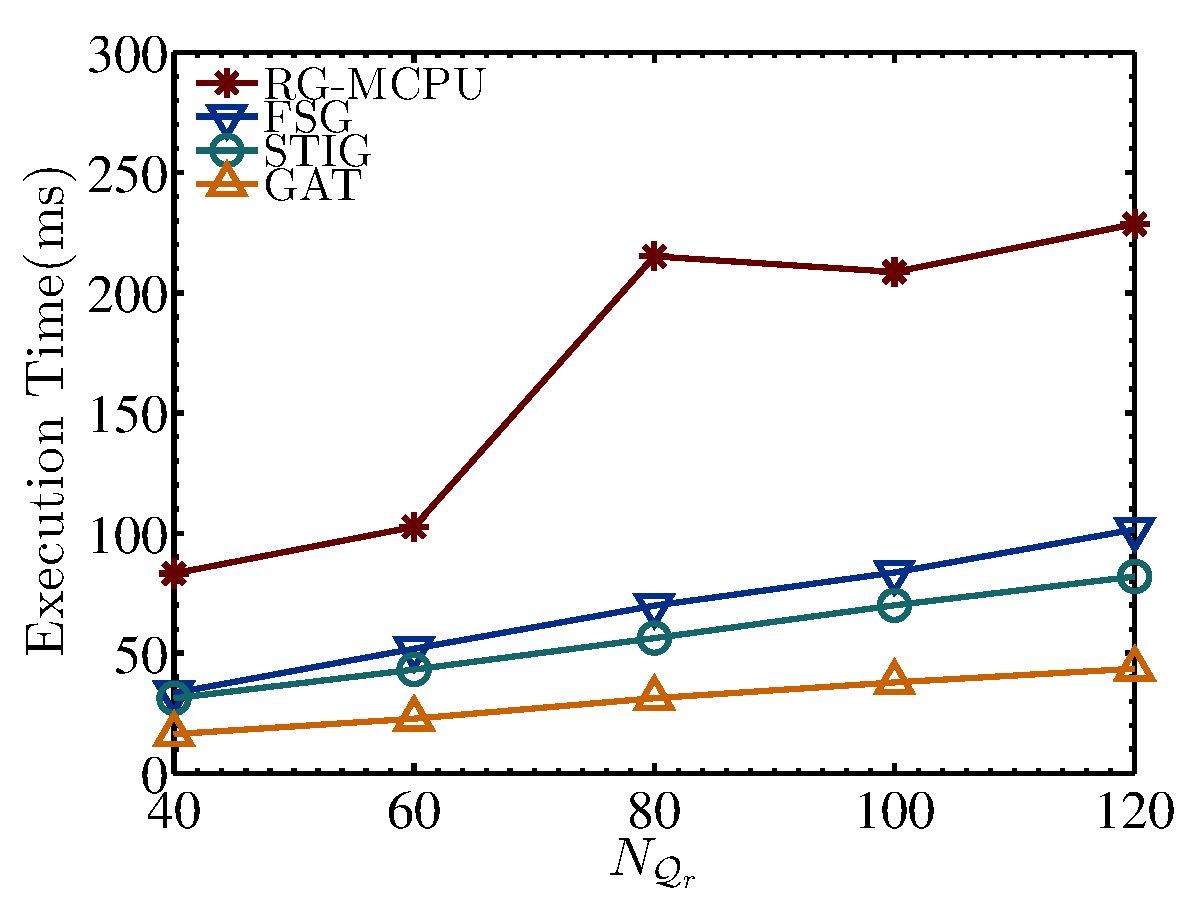
\includegraphics[width=\linewidth,height=2.9cm]{eps/QueryNum_RangeQ.eps}
			(a) SHCAR
		\end{minipage}
		\hfill
		\begin{minipage}{0.48\linewidth}
			\centering
			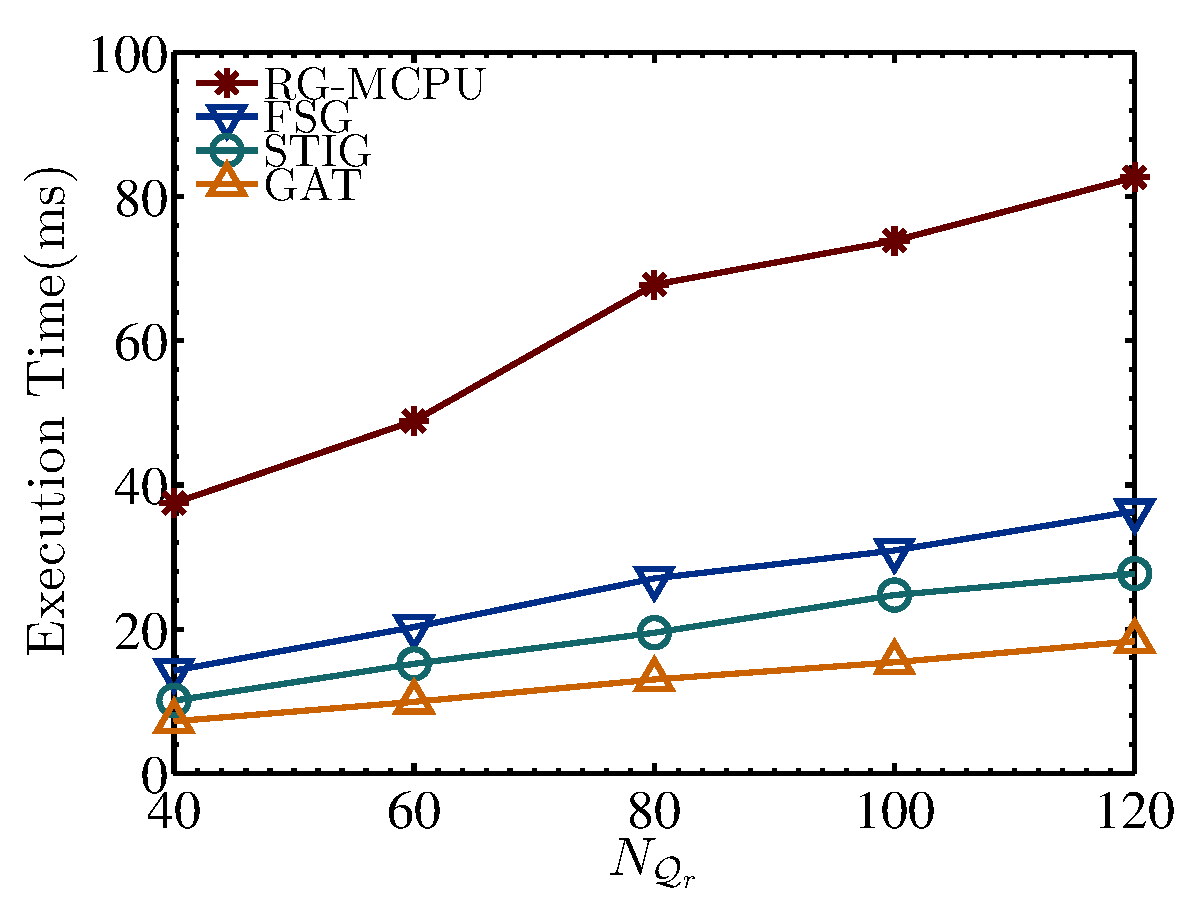
\includegraphics[width=\linewidth,height=2.9cm]{eps/QueryNum_RangeQ_GEO.eps}
			(a) GeoLife
		\end{minipage}	
	}
	\caption{Comparison of performance on range queries \label{fig:QueryNum_range}}
	\vspace{-.1in}
\end{figure}

\begin{figure}[!t]\centering
	\scriptsize{
		\begin{minipage}{0.48\linewidth}
			\centering
			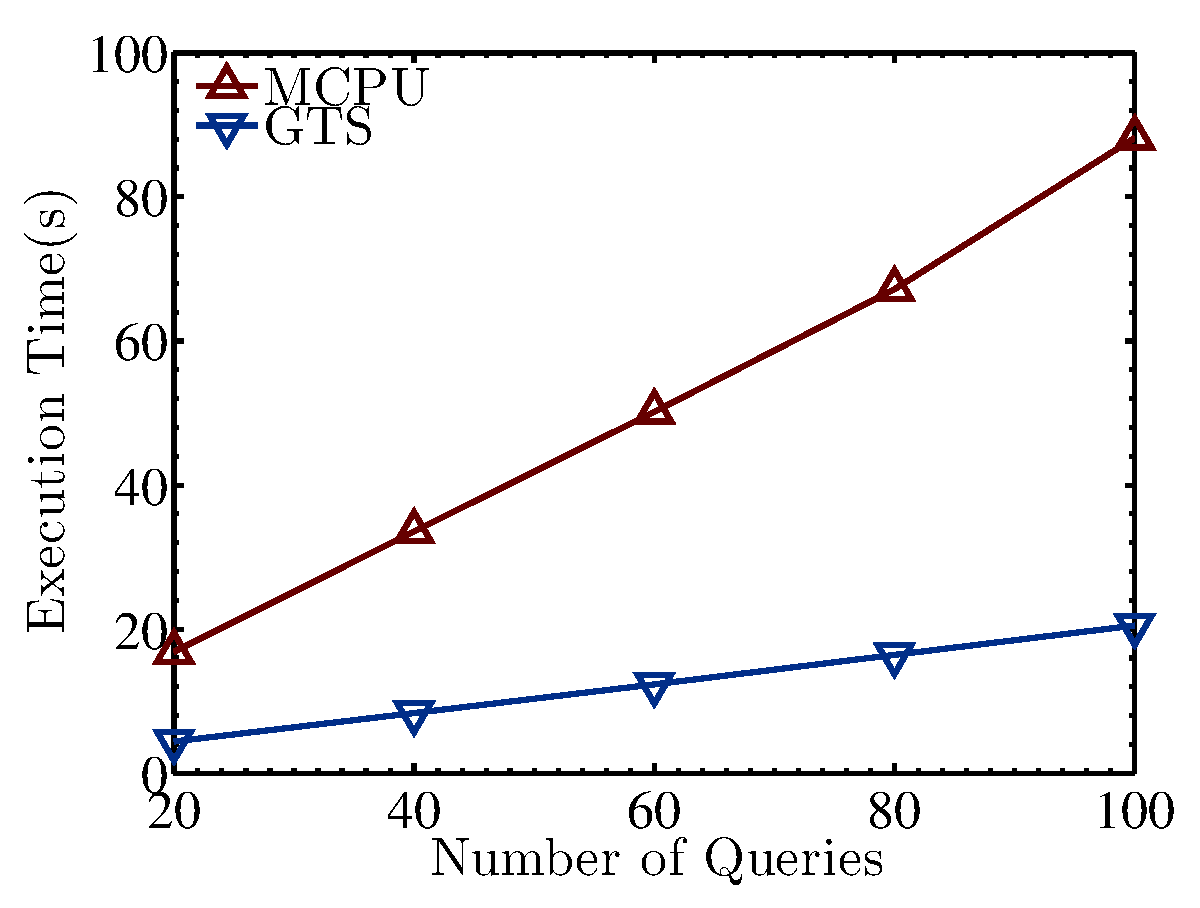
\includegraphics[width=\linewidth,height=2.9cm]{eps/QueryNum_SimilarityQ.eps}
			(b) SHCAR
		\end{minipage}
		\hfill
		\begin{minipage}{0.48\linewidth}
			\centering
			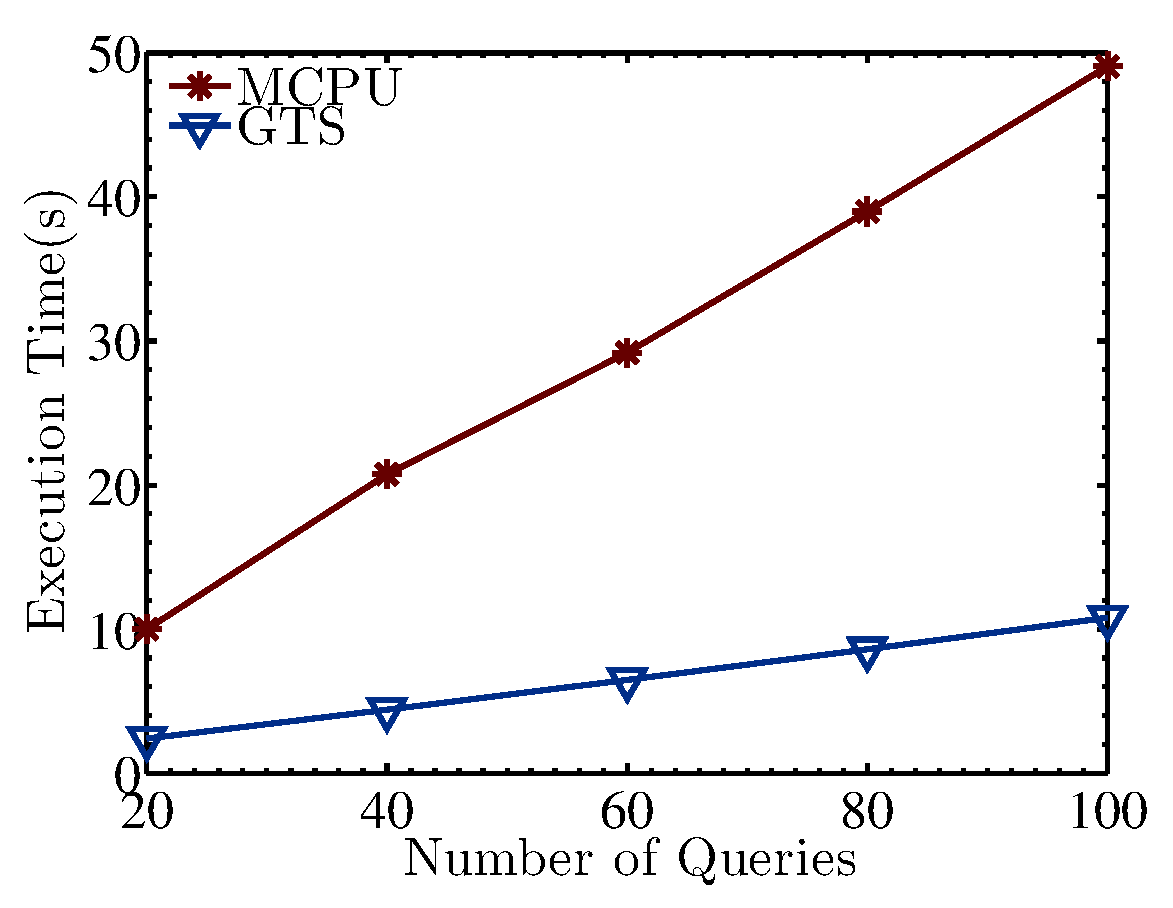
\includegraphics[width=\linewidth,height=2.9cm]{eps/QueryNum_SimilarityQ_GEO.eps}
			(b) GeoLife
		\end{minipage}
	}
	\caption{Comparison of performance on similarity queries \label{fig:QueryNum_sim}}
	\vspace{-.1in}
\end{figure}
\begin{figure}[!t]\centering
	\scriptsize{
		\begin{minipage}{0.48\linewidth}
			\centering
			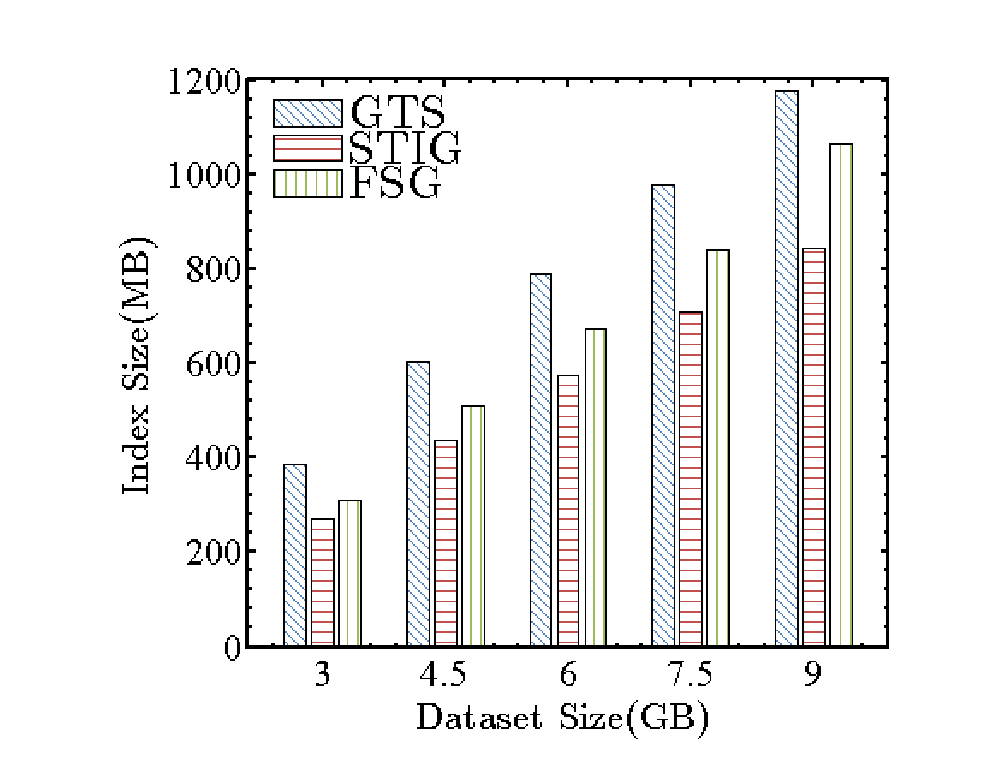
\includegraphics[width=\linewidth,height=2.9cm]{eps/indexSize.eps}
			(a) Memory Cost
		\end{minipage}
		\hfill
		\begin{minipage}{0.48\linewidth}
			\centering
			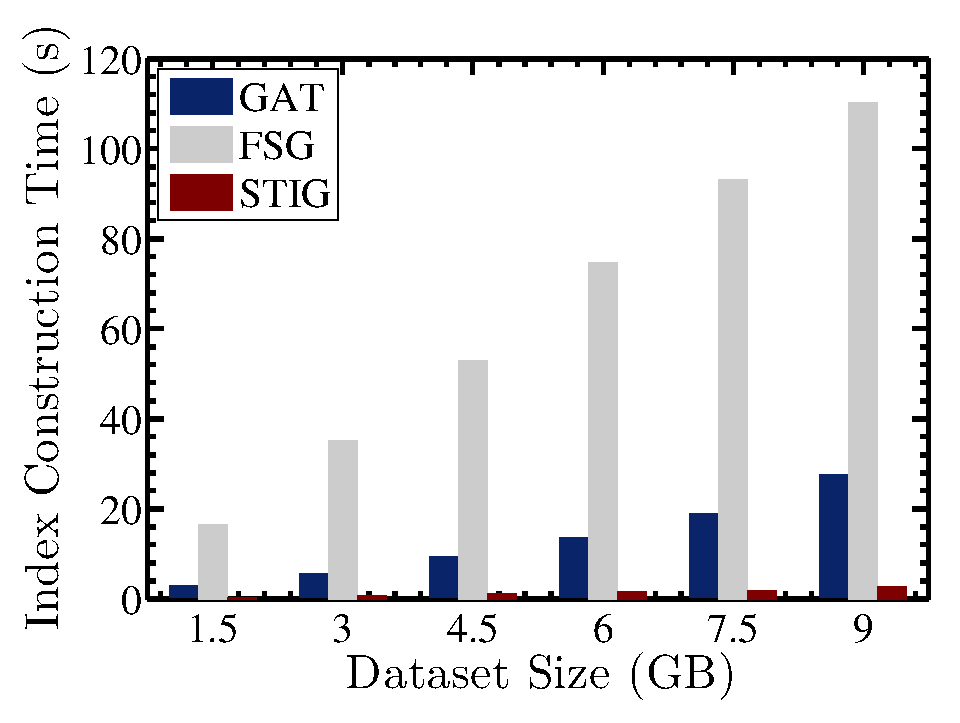
\includegraphics[width=\linewidth,height=2.9cm]{eps/indexTime.eps}
			(b) Index Construction Time
		\end{minipage}
	}
	\caption{Indexing cost\label{fig:IndexCost}}
	\vspace{-.1in}
\end{figure}

We evaluate indexing cost for three GPU approaches. We randomly select subsets of trajectories from both SHCAR and GeoLife, and build indices for each subset.
% The result are shown in Figure~\ref{fig:IndexCost}.
%All the parameters are set to default.

\vspace{0.1cm}\textbf{Memory Cost.}
Figure~\ref{fig:IndexCost}(a) shows the index memory cost w.r.t. different data sizes.
For all the approaches, the size of indices becomes larger when the data size increases.
\frname requires slightly more memory cost ($8$\%-$29$\%) compared with other two methods.
%There is a small increment ($8$\%-$29$\%) of memory cost in \frname compared to other two methods.
The main reason is that \frname involves trajectory index to perform histogram-based pruning for similarity queries, while STIG and FSG can only process range queries and do not maintain such an index.
On average, the overhead of \idxname is merely $12.8$\% of the data size, which is acceptable and space-efficient.
%In the evaluation of $9$GB dataset only about $80$MB to $290$MB more memory is consumed compared to FSG ($1063$MB) and STIG ($853$MB), it is an acceptable cost considering the big increment on throughput in \frname.

\vspace{0.1cm}\textbf{Index Construction Time.}
Figure \ref{fig:IndexCost}(b) provides the index construction time for different data sizes.
The construction time increases as the data size becomes large. For 9GB data, \frname takes only $27.7$ seconds for index construction, which is efficient.
\frname requires $75.2$\% less index construction time than STIG over all the data sizes. This is because STIG needs to compute a large number of medium values when generating kd-tree.
The index construction time of \frname is longer than that of FSG due to the additional tree index $\treeindex$ in \frname.


\subsection{Speedup}

We next study the speedup achieved by \frname with default parameter values on one and two GPUs. For comparison, we use a single thread to execute all the queries on CPU. The speedup is computed as the ratio of execution time against the single-thread approach.
%This study explains two benefits. First, it shows that our GPU-based implementation can outperform traditional implementation on CPU. Second, it demonstrates that a near-linear improvement of efficiency can be achieved by adding more GPU devices.
Table \ref{tab:speedup} shows the results on two datasets.
%
For range queries, \frname with one GPU achieves $20.07$x and $18.03$x speedups on SHCAR and GeoLife respectively, owning to the high parallelism of GPU. Using two GPUs achieves about $1.76$x speedup than using one GPU over both datasets. This indicates that \frname can achieve almost linear speedup with more GPUs.
%
For similarity queries, \frname with one GPU achieves $35.54$x and $38.94$x speedups on SHCAR and GeoLife, respectively. The speedups are higher than those for range queries. Compared with similarity queries, range query processing involves simple comparison operations and the data transfer cost between main memory and global memory may become more significant in the overall execution time, which restricts the increase of speedup.

%Our approach achieves up to $38.94$ speedup in evaluation of top-$k$ similarity query for single GPU, and 74.95x in dual GPUs environment. The high speedup ratio comes from the parallel execution of compute-intensive EDR calculation.
%For range query, a lower speedup ratio of 20.07x for single GPU and 37.63x for dual GPUs is achieved. Considering that only some comparison operations need to be performed in verification procedure, the larger propotion of data transfering cost restricts the speedup ratio compared to similarity query.


\begin{table}[t]
	\centering
	
	\caption{Speedup achieved on two datasets}     % NOTE!  caption goes _before_ the table contents !!
	\label{tab:speedup}
	\vspace{-.1in}
	\scriptsize{
		\begin{tabular}{|l|c|c|c|c|}
			\hline
			{\bfseries Dataset} & \multicolumn{2} {c|} {\bfseries SHCAR} & \multicolumn{2} {c|} {\bfseries GeoLife} \\
			\cline{1-5}
			{\bfseries \#GPUs} & {\bfseries 1GPU} &  {\bfseries 2GPU}  & {\bfseries 1GPU} &  {\bfseries 2GPU}  \\
			\hline
			Range Query & 20.07 & 37.63 & 18.03 & 32.43 \\
			\hline
			Top-k Similarity Query & 35.54 & 68.53 & 38.94 & 74.95 \\
			\hline
		\end{tabular}
	}
\vspace{-.1in}
\end{table}



\subsection{Scalability}

%Figure~\ref{fig:Scalability} presents the results under different size of data in the range from $3$GB to $9$GB.



We investigate the scalability of different approaches by varying the data size from $3$GB to $9$GB.
%\vspace{0.1cm}\textbf{Range Query.}
Figure~\ref{fig:Scalability}(a) shows the execution time of 80 range queries over different data sizes. All the approaches require longer execution time when the dataset becomes larger. This is determined by the fact that large datasets typically involve more candidates to be verified.
\frname scales better than FSG, as \frname groups cells into blocks to achieve load balancing.
%in \frname the effect of the skew dataset is mitigated owing to the similar-sized blocks in quadtree-like index in \idxname, while FSG suffers from unbalanced workloads on different GPU SMs caused by different number of points in each cell of the flat grid-file based index.
This phenomenon is more significant on larger datasets, which limits the scalability of FSG.
%shenyy: fillin
%
%However, as the growing scale of dataset, the execution time on GPU-based methods show a sub-linear increasing trend. This is because the increment of more expensive data transferring between main memory and GPU is quicker than that of quantity of candidates waiting for verification.\textbf{Why?????????}
%We can also see our approach performs better when facing large scale dataset than other GPU-based baselines, indicating that our system has a good scalability on range query.
%
%\vspace{0.1cm}\textbf{Similarity Query.}
Figure~\ref{fig:Scalability}(b) reports the execution time of similarity queries over different data sizes. As data volume grows, both \frname and \frname-CPU-S require longer execution time. However, the execution time of \frname grows much slower than that of \frname-CPU-S, indicating better scalability using the GPU.
% two approaches consume more time on queries and the benefit of acceleration by using GPU becomes more obvious. It also proves that our system works excellently on large-scale dataset.


\subsection{Parameter Tuning}

In this section, we study the effects of different parameter values on the performance of \frname, as listed in Table~\ref{table_param}.
%Some of them can be categorized as query parameters, which are properties of queries and can be evaluated in both other systems and GTS, such as the area of MBR and $k$. Others are system parameters, which only exist in our system. For this reason, we show results of all baselines when evaluating the execution time in different query conditions to demonstrate both the expected performance in various environment and the effects of these parameters. Meanwhile, system parameters are evaluated under different query scales to show the effects, which are only based on our approach.

%\vspace{0.1cm}\textbf{Range Query.}~~There are three parameters about range query: $S_R$, $\theta_p$ and $n$. We will evaluate the effects of them.



% zbw: in this part the unit of area can be transfromed into standard unit
\vspace{0.1cm}\textbf{Effect of query region area $S_R$ ($km^2$).}
The area of query region $S_{R}$ controls the selectivity of range query. All the query regions are generated by extending from a point in the city center. Figure~\ref{fig:RANGE} shows the results with different $S_{R}$.
The execution time of all approaches increases when the area of $R$ varies from $10km^2$ to $40km^2$.
%shenyy: show unit in figures.
As the query region becomes larger, more blocks overlap with $R$, leading to more candidates for verification.
\frname performs the best over all the areas on GeoLife, but runs slightly slower than FSG for $S_R=10km^2$ on SHCAR. The reason may be that SHCAR involves a small number of points residing in a small query region, but \frname verifies the whole block if any of its cells is overlapped with $R$.
%However, in FSG, only points in cells which overlap $R$ need to be checked whether they are within $R$.
%On average, \frname runs $?$x and $?$x faster than STIG and FSG, respectively.
The GPU solutions outperform \frname-CPU-R in all cases, due to the superior of the GPU in parallel computations.

%We can see that this trend is nearly linear for our framework, because the scale of verification and the number of nodes overlapped by query region $R$ are basically propotional to the area of it.
%Our frameworks shows a better throughput even in the query region with a large area.

\begin{figure}[t]\centering
	\scriptsize{
		\begin{minipage}{0.48\linewidth}
			\centering
			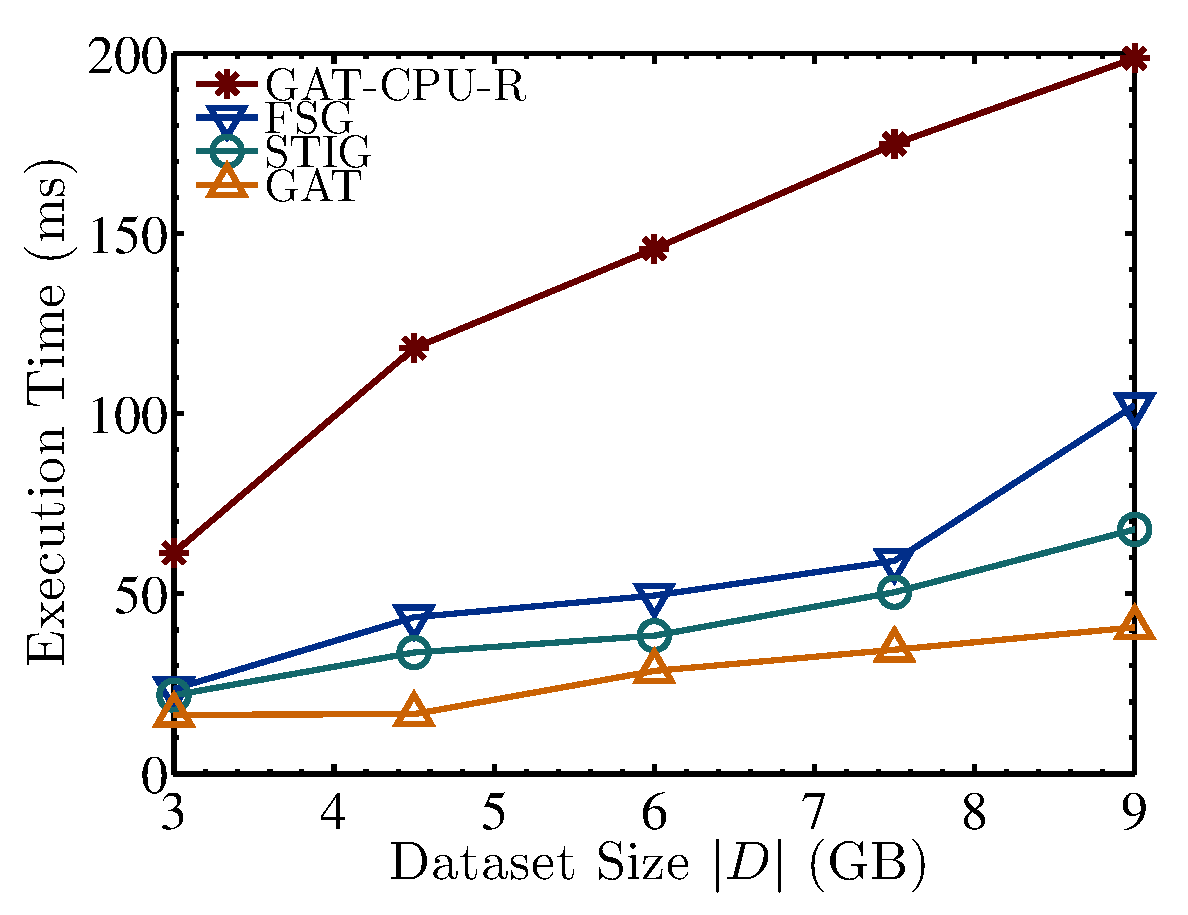
\includegraphics[width=\linewidth,height=2.9cm]{eps/range_scala.eps}
			(a) Range Query
		\end{minipage}
		\hfill
		\begin{minipage}{0.48\linewidth}
			\centering
			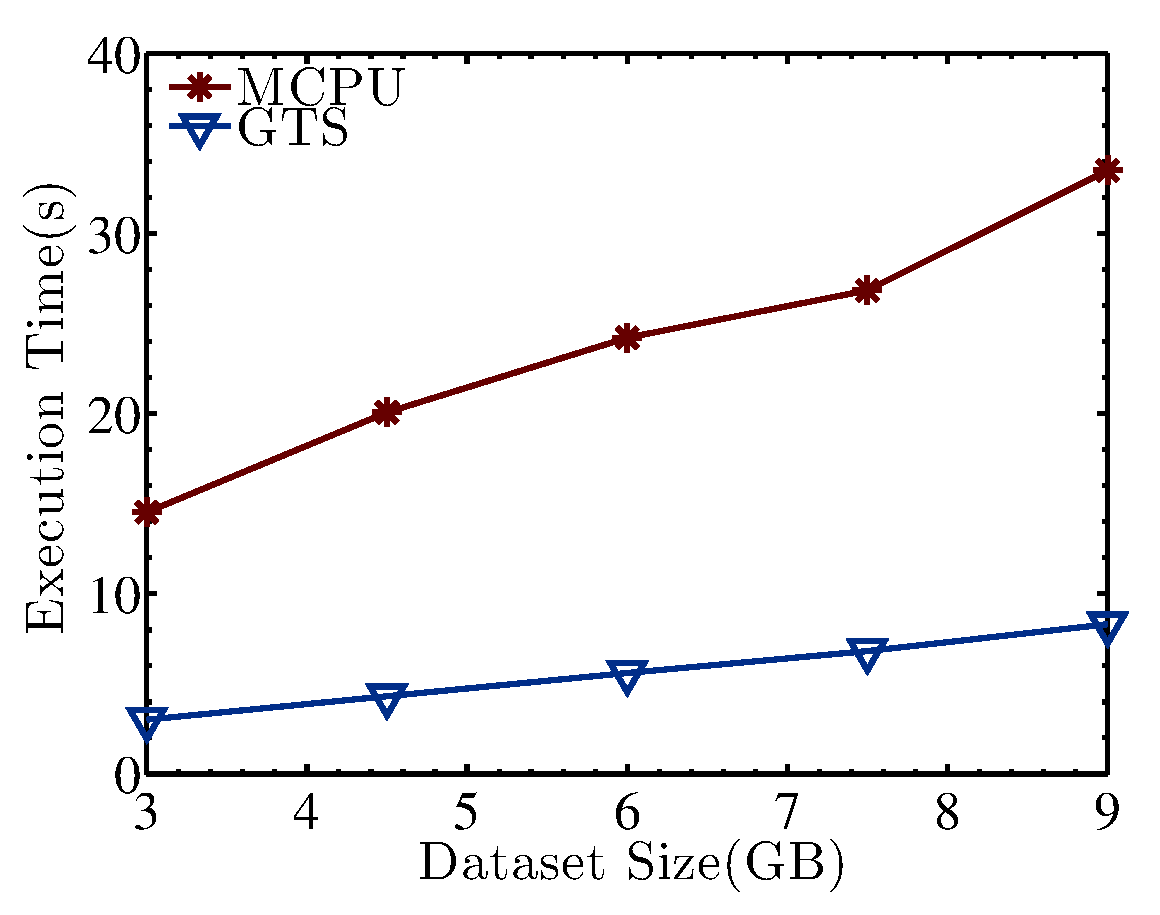
\includegraphics[width=\linewidth,height=2.9cm]{eps/similarity_scala.eps}
			(b) Similarity Query
		\end{minipage}
	}
	\caption{Scalability\label{fig:Scalability}}
	\vspace{-.1in}
\end{figure}

\begin{figure}[!t]\centering
	\scriptsize{
		\begin{minipage}{0.48\linewidth}
			\centering
			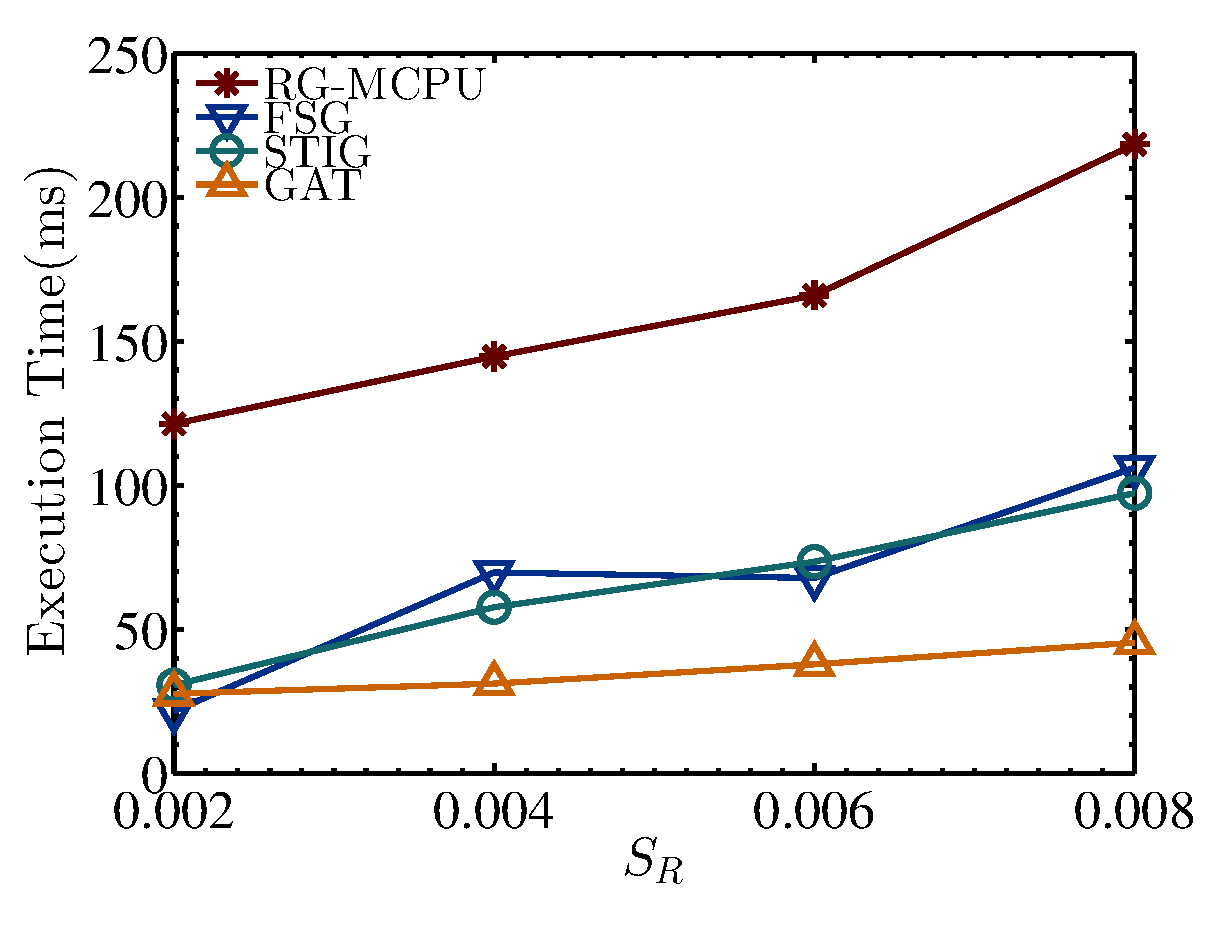
\includegraphics[width=\linewidth,height=2.9cm]{eps/RangeArea.eps}
			(a) SHCAR
		\end{minipage}
		\hfill
		\begin{minipage}{0.48\linewidth}
			\centering
			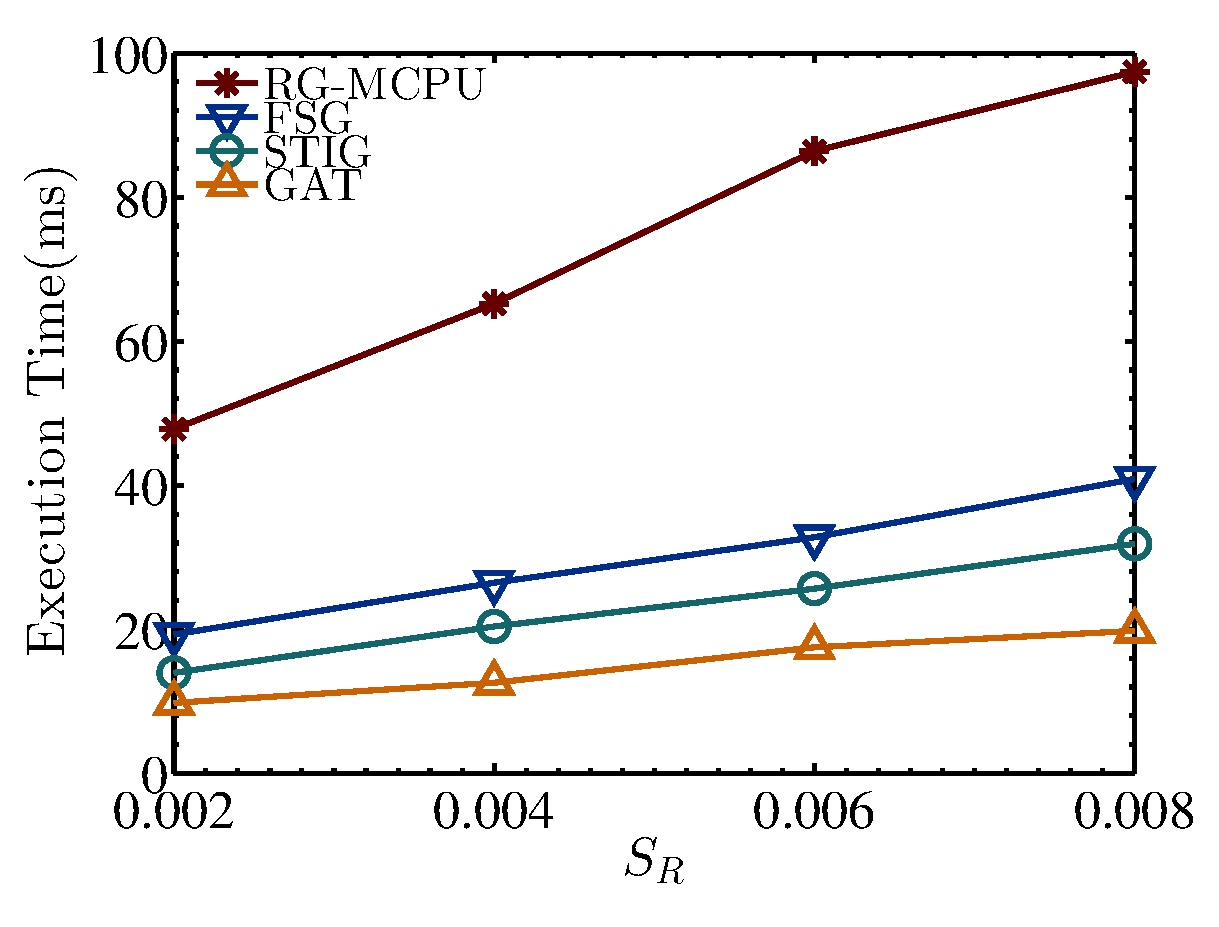
\includegraphics[width=\linewidth,height=2.9cm]{eps/RangeArea_GEO.eps}
			(b) GeoLife
		\end{minipage}
	}
	\caption{Effect of query region area ($S_R$) \label{fig:RANGE}}
	\vspace{-.1in}
\end{figure}
\begin{figure}[t]\centering
	\scriptsize{
		\begin{minipage}{0.48\linewidth}
			\centering
			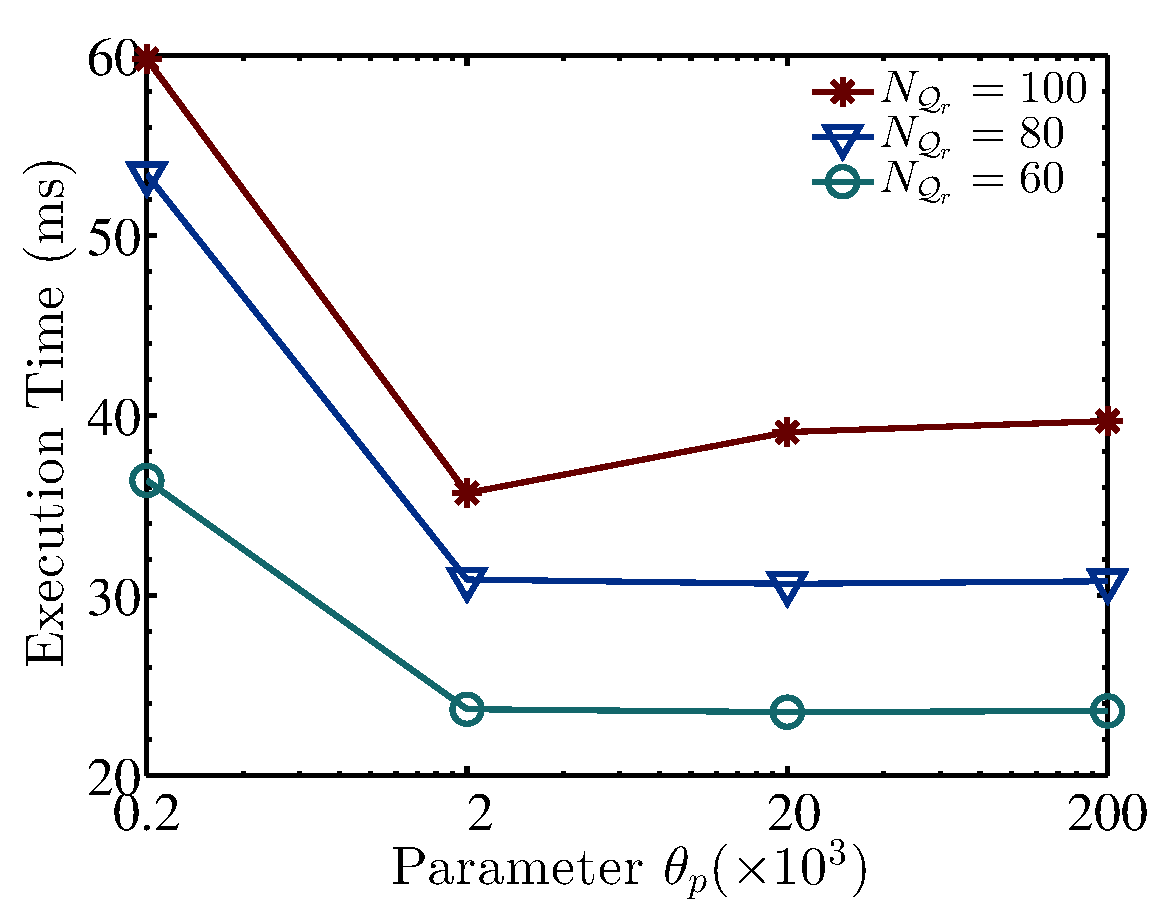
\includegraphics[width=\linewidth,height=2.9cm]{eps/MCELL.eps}
			(a) SHCAR
		\end{minipage}
		\hfill
		\begin{minipage}{0.48\linewidth}
			\centering
			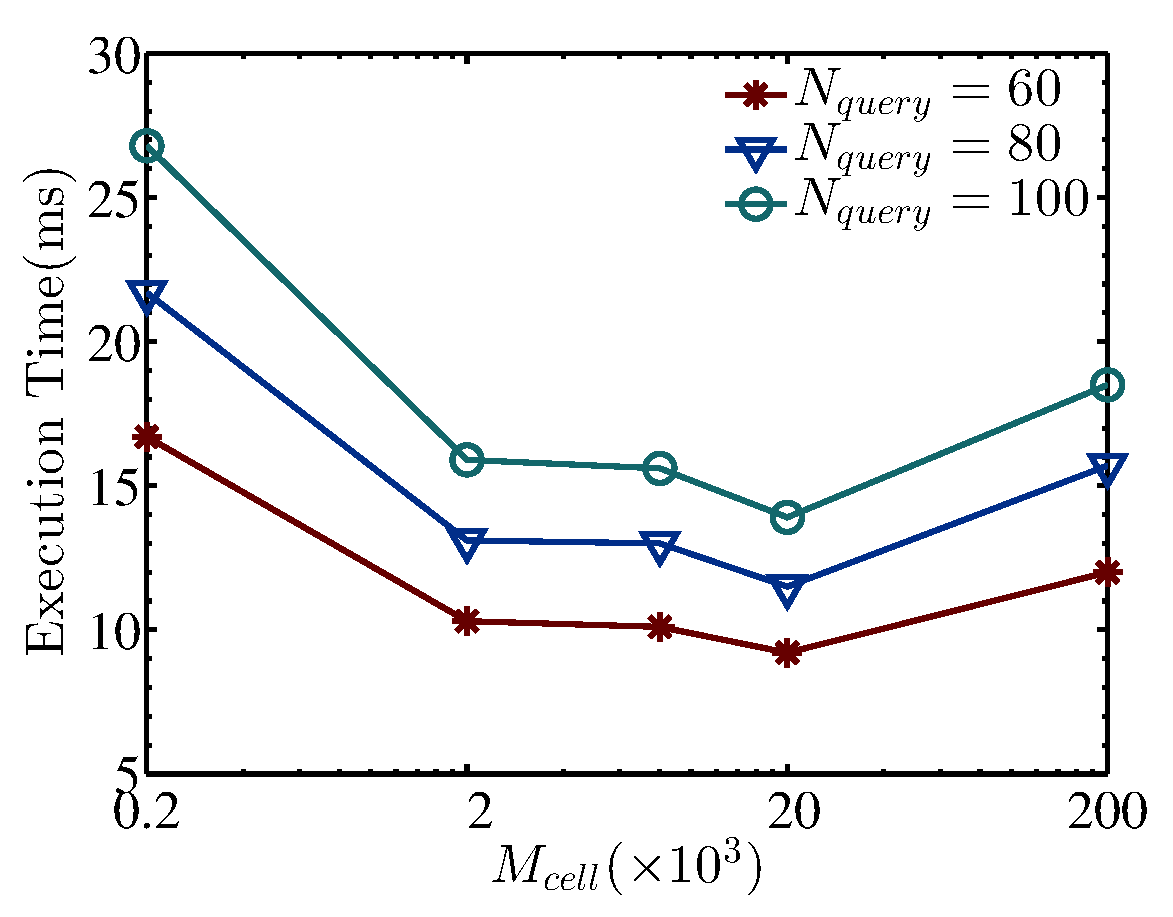
\includegraphics[width=\linewidth,height=2.9cm]{eps/MCELL_GEO.eps}
			(b) GeoLife
		\end{minipage}
	}
%	\vspace{-.03in}
	\caption{Effect of block size threshold ($\theta_p$) \label{fig:MCELL}}
	\vspace{-.1in}
\end{figure}

\vspace{0.1cm}\textbf{Effect of block size threshold $\theta_p$.}
%shenyy: remove theta_p=8000 in the figures
Figure \ref{fig:MCELL} shows the execution time of range queries with various values of $\theta_p$. Recall that a large value of $\theta_p$ means that more cells are grouped into a large block, while the total number of blocks is reduced.
%shenyy:explain
%of $N_{\rangeq}=60$, $N_{\rangeq}=80$ and $N_{\rangeq}=100$.
For both datasets, we observe that the execution time of \frname decreases significantly when $\theta_p$ varies from $200$ to $2000$.
%, and then becomes stable for larger values of $\theta_p$.
When $\theta_p$ is too small, the number of points per block becomes smaller and verifying a few points in a candidate block cannot fully utilize the parallelism of GPU SM.
We also observe a slight increase in execution time when $\theta_p$ varies from $20,000$ to $200,000$. This is because larger $\theta_p$ results in more points per block and the size difference among blocks becomes larger. Such variance causes unbalanced workloads.


%We can see under about $\theta_p=8000$ and $\theta_p=20000$ our approach achieves the best performance on both datasets respectively.
%There is a downward trend of execution time as decreasing $\theta_p$, because if $\theta_p$ is too small, each SM of GPU need only finish several comparison operations between points and the query region (e.g., less than the number of cores in SM), leading to not fully usage of GPU.
%On the other hand, in the result of Geolife, as $\theta_p$ continues to increase from $20000$, the execution time goes up slightly. This is because the workload of verification tasks on each SM becomes extremely large, so the absolute gap among the cost of each task is indeed bigger, leading to an unbalanced workload.

\begin{figure}[!t]\centering
	\scriptsize{
		\begin{minipage}{0.48\linewidth}
			\centering
			\includegraphics[width=\linewidth,height=2.9cm]{eps/n_filter.eps}
			(a) SHCAR
		\end{minipage}
		\hfill
		\begin{minipage}{0.48\linewidth}
			\centering
			\includegraphics[width=\linewidth,height=2.9cm]{eps/n_FD.eps}
			(b) GeoLife
		\end{minipage}
	}
	\caption{Effect of maximum quadtree level ($n$) \label{fig:LCELL}}
	\vspace{-.1in}
\end{figure}


\vspace{0.1cm}\textbf{Effect of maximum quadtree level $n$.}
The value of $n$ controls the number of cells in $\allcell$. As we use $\theta_p$ to group cells into blocks, the performance of \frname on range queries is quite stable with different $n$. We thus omit the results due to the space limit.
Figure~\ref{fig:LCELL} provides the execution time of similarity queries on two datasets by varying $n$. As $n$ increases, calculating frequency distance requires more execution time. The reason is that the length of FV is exponential to $n$ and the computational cost of FD is linear to the length of FV. The time of the iterations for generating candidates and calculating EDR decreases as $n$ becomes larger, because more cells lead to tighter lower bounds of EDR and stronger pruning power.
%shenyy: use new figures!!
%Figure \ref{fig:LCELL} shows the result when parameter $n$ varying from $7$ to $10$, noting that with the restriction that $\theta_p=20000$, $n$ has to be set larger than $7$, or the number of points in some cells will exceed $20000$.
%%We can see the there is only slight change of performance. This is because the cells are grouped into blocks during filtering phase as the unit of task assignment, so the change of the number and size of cells do not affect the task division and verification scale in each SM significantly, which are the main factors of the performance.
%In SHCAR, execution time of range queries decrease mildly as the larger $n$, because in this situation a more fine-grained division of cells are performed, then through grouping cells into blocks the number of points in each block becomes more balance.
%However, in GeoLife, the execution time increase slightly under larger $n$. This may be because in some dense area fine-grained cells directly form the leaf nodes in level $n$ of $\treeindex$, leading to a greater depth in these branches and then more cost of filtering.

%\vspace{0.1cm}\textbf{Similarity Query.}~~In this section, we study the effects of parameters in top-$k$ similarity query, including $k$ and $\zeta$.




\vspace{0.1cm}\textbf{Effect of $k$.}
Figure~\ref{fig:kValue} shows the execution time of similarity queries under different values of $k$. As $k$ becomes larger, both \frname and \frname-CPU-S require longer execution time. This is because larger $k$ requires more EDR distances to be computed.
However, for \frname, the increase in the execution time is small as the EDR computations are performed by thousands of GPU cores and the extra cost with larger $k$ can be amortized.


%We can see that for all $k$ values our approach achieves better performance than CPU-based implementation.
%In both two approaches, execution time goes higher as the $k$ value increases. This is because under a larger $k$ more EDR should be calculated before reaching terminate condition. The amplitude of increment in the number of EDR calculation becomes smaller as $k$ grows, so the execution time tends to be constant after $k$ is large enough.

\begin{figure}[t]\centering
	\scriptsize{
		\begin{minipage}{0.48\linewidth}
			\centering
			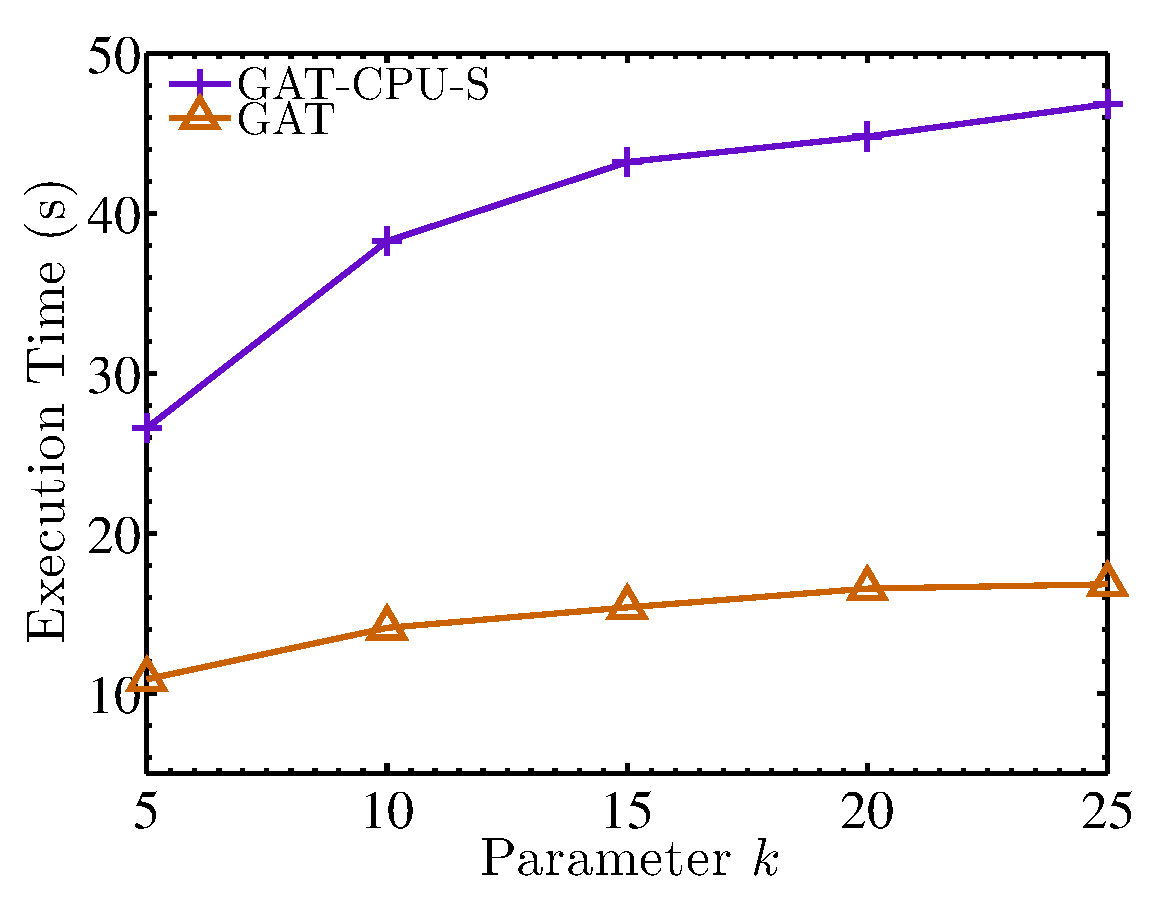
\includegraphics[width=\linewidth,height=2.9cm]{eps/kValue.eps}
			(a) SHCAR
		\end{minipage}
		\hfill
		\begin{minipage}{0.48\linewidth}
			\centering
			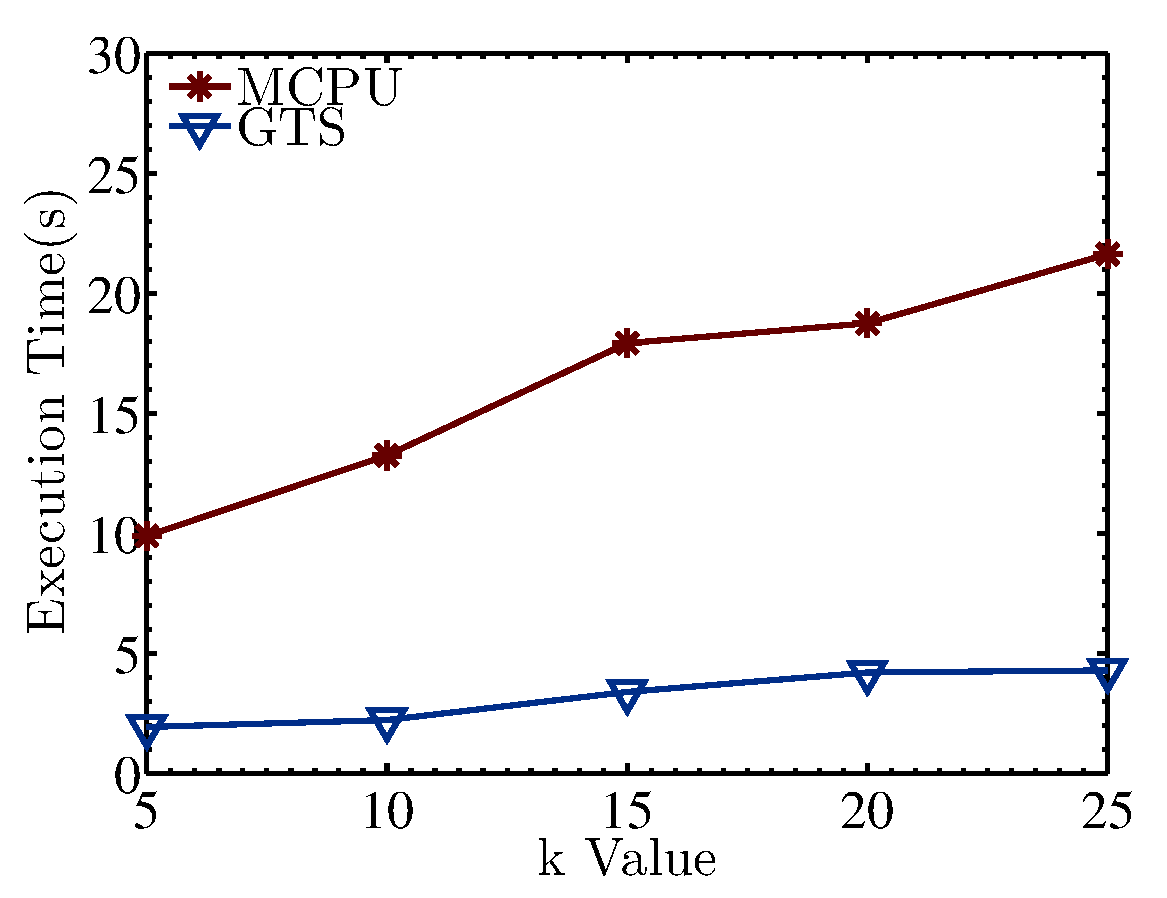
\includegraphics[width=\linewidth,height=2.9cm]{eps/kValue_GEO.eps}
			(b) GeoLife
		\end{minipage}
	}
%	\vspace{-.1in}
	\caption{Effect of $k$ \label{fig:kValue}}
	\vspace{-.1in}
\end{figure}

\begin{figure}[t]\centering
	\scriptsize{
		\begin{minipage}{0.48\linewidth}
			\centering
			\includegraphics[width=\linewidth,height=2.9cm]{eps/trajLength.eps}
			(a) SHCAR
		\end{minipage}
		\hfill
		\begin{minipage}{0.48\linewidth}
			\centering
			\includegraphics[width=\linewidth,height=2.9cm]{eps/trajLength_GEO.eps}
			(b) GeoLife
		\end{minipage}
		%%shenyy: replace with a new graph
	}
	\caption{Effect of query trajectory length ($\zeta$) \label{fig:LENSIMI}}
	\vspace{-.1in}
\end{figure}

\vspace{0.1cm}\textbf{Effect of average query trajectory length $\zeta$.}
We study the effect of average query trajectory length on similarity query processing. For each length, we randomly choose $50$ trajectories and report the averaged result.
Figure~\ref{fig:LENSIMI} shows the results.
For both SHCAR and GeoLife, \frname outperforms \frname-CPU-S over all the trajectory lengths.
The reason is that \frname computes each EDR distance with one SM and the computational cost is proportional to the sum of two trajectory lengths in our proposed algorithm.
% with multi the amount of computation in EDR calculation is only the same as the number of iterations for computing states in parallel for an SM, which is almost equal to the addition of the query trajectory length $\zeta$ and the candidate trajectory length.
However, \frname-CPU-S adopts the original dynamic programming method and the complexity of computing EDR distance is proportional to the multiplication of two trajectory lengths.
The advantage of \frname thus becomes more significant for larger $\zeta$.





%%%%%%%%%%%%%%%%%%%%%%%%%%%%%%%%%%%%%%%%%%%%%%%%%%%%%%%%%%%%%%%%%%%%%%%%%%%%%%%%%%%%%%%%%%%%%%
\section{Related Work}\label{sec:related}

We review related works divided into two categories: trajectory indexing and GPU-based trajectory query processing.

\vspace{0.1cm}{\bf Trajectory indexing.}
%
R-Tree~\cite{DBLP:conf/sigmod/Guttman84} is one of most classical indices for spatial data, which is a two-dimensional generalization of B-Tree~\cite{DBLP:conf/sigmod/BayerM70}.
After that, some indices such as 3D-RTree~\cite{DBLP:conf/icmcs/TheodoridisVS96}, TB-Tree~\cite{DBLP:conf/vldb/PfoserJT00} and TPR-Tree~\cite{DBLP:conf/sigmod/SaltenisJLL00} have been proposed to index trajectory data.
% However, they are non-adaptive, meaning that they suffered from a performance loss as the diversity of trajectory distribution.
SETI~\cite{DBLP:conf/cidr/ChakkaEP03} proposed a two-level indexing scheme by decoupling spatial and temporal dimensions for spatial queries.
PIST~\cite{DBLP:journals/geoinformatica/BoteaMNS08} developed a cost model to measure the IO cost of different partitioning over spatial-temporal data, in order to reduce the number of disk accesses.
TrajStore~\cite{DBLP:conf/icde/Cudre-MaurouxWM10} proposed an adaptive griding scheme for indexing, clustering and storing trajectory data.
Wang et al. developed an in-memory column-oriented storage called SharkDB~\cite{DBLP:conf/cikm/WangZXZZS14} for trajectories, where range and similarity queries can be executed in memory efficiently.
Trajtree~\cite{EDWP15} was designed to index the computation of EDwP, a similarity metric for trajectories under inconsistent sampling rates.
All these indexing schemes are designed for spatial query processing on CPU, which can be incorporated into the filtering part of our framework. However, they are not optimized for GPU-accelerated verification, thus inspiring us to develop \idxname.
%, so throughput in them under big trajectory dataset is limited comparing to our \frname framework.

\vspace{0.1cm}{\bf GPU-based trajectory query processing.}
%
The GPU has been used for accelerating query processing over trajectory data. Zhang et al.~\cite{Zhang:2012:USH} proposed a system called U$_2$STRA to manage large-scale trajectory data efficiently on GPU. They proposed to split trajectories with a four-level hierarchy and index them by a grid-file based data structure. Based on this system, an algorithm called TKSimGPU~\cite{DBLP:conf/bigdataconf/LealGZY15} was developed for top-$k$ similarity queries. The idea is to compute similarity for pairs of trajectories using GPU.
%It calculate Hausdorff distance between two trajectories by distributing the tasks of computing the distance of subsequences in different cells to GPU cores and then merge the results.
However, this approach adopted Hausdorff distance as the similarity measure, which is not robust to noise in real trajectories. And the solution cannot support more accurate similarity metrics such as EDR distance~\cite{DBLP:conf/sigmod/ChenOO05}.
%It calculate Hausdorff distance between two trajectories by distributing the tasks of computing the distance of subsequences in different cells to GPU cores and then merge the results.
%However, TKSimGPU failed in the supporting of some popular and robust distance functions such as EDR~\cite{DBLP:conf/sigmod/ChenOO05}, DTW~\cite{DBLP:conf/vldb/Keogh02} and EDwP~\cite{EDWP15}, because the task division strategy of it only support considering matching points within one cell in a subtask.
%However, Hausdorff is not as popular and robust as the distance functions based on global alignment such as EDR~\cite{DBLP:conf/sigmod/ChenOO05}, DTW~\cite{DBLP:conf/vldb/Keogh02} and EDwP~\cite{EDWP15}, requiring all the matching cases of any two points in whole trajectories are considered during the computation. Therefore the task division strategy of TKSimGPU failed in these distance funcitons because only points within the cell can be used in a subtask.
%For another thing, the grid-file based data structure will suffer from unbalanced load when the distribution of dataset is not uniform, because the quantities of points in different cells differ dramatically.
%
Lettich et al.~\cite{DBLP:conf/gis/LettichOS15} proposed the PR-quadtree to process stream spatial $k$-nearest neighbor queries, where a PR-quadtree index was developed to achieve load balancing in query processing.
However, they require to load all the data into global memory for processing, which cannot scale to large datasets.
%But different from our \frname framework, both index construction and query processing are finished in the GPU in this work, because the scale of stream spatial data is usually not so large and they can be fully loaded into global memory.
Zhang et al.~\cite{GPUTaxi} developed a query processing system with a grid-file based data structure to manage taxi trips.
Doraiswamy et al.~\cite{7498315} generalized the kd-tree to STIG in order to support iterative spatial-temporal queries using the GPU.
However, these approach does not support trajectory similarity queries and the performance on range queries is inferior to GAT.

%
%\section{Related Work}\label{sec:related}
%
%In this sectoin we review some previous related works about Trajectory Indexing and GPU-accelerated Spatial Query Processing.
%
%\subsection{Trajectory Indexing}
%
%R-Tree~\cite{DBLP:conf/sigmod/Guttman84} is the most classical index for spatial data, which is the two-dimensional generalization of B-Tree~\cite{DBLP:conf/sigmod/BayerM70}.
%After that some indices optimized for trajectory such as 3D-RTree~\cite{DBLP:conf/icmcs/TheodoridisVS96}, TB-Tree~\cite{DBLP:conf/vldb/PfoserJT00} and TPR-Tree~\cite{DBLP:conf/sigmod/SaltenisJLL00}. They index on the temporal dimension as well as the spatial dimension.
%% However, they are non-adaptive, meaning that they suffered from a performance loss as the diversity of trajectory distribution.
%SETI~\cite{DBLP:conf/cidr/ChakkaEP03} proposed a indexing mechanism which forms a two-level index by decoupling the spatial dimension and temporal dimension to reduce the complexity of spatial query.
%PIST~\cite{DBLP:journals/geoinformatica/BoteaMNS08} developed a cost model of partitioning the data space for different data distributions, aiming to reduce the number of disk accesses.
%TrajStore~\cite{DBLP:conf/icde/Cudre-MaurouxWM10} proposed an adaptive algorithm to split trajectories optimally and cluster them physically to achieve a lowest expected I/O cost.
%Wang et.al. developed an in-memory column-oriented storage called SharkDB~\cite{DBLP:conf/cikm/WangZXZZS14} to achieve the high performance in range queries and kNN queries and avoid the expensive I/O operations.
%Trajtree~\cite{EDWP15} was designed to index the computation of EDwP, a similarity metric optimized for trajectories under inconsistent sampling rates.
%However, these works are all designed to process queries on CPU, so throughput in them under big trajectory dataset is limited comparing to our \frname framework.
%
%\subsection{GPU-accelerated Spatial Query Processing}
%GPU has been used for accelerating the query processing for both spatial-temporal data including trajectory. Zhang et.al~\cite{Zhang:2012:USH} proposed a prototype system called U$_2$STRA to manage large-scale trajectory data efficiently using GPU. It proposed a four-level hierarchy to split and represent trajectories, and then index them by a grid-file based data structure. Based on this system, a top-$k$ similarity query algorithm called TKSimGPU~\cite{DBLP:conf/bigdataconf/LealGZY15} is developed. It calculate Hausdorff distance between two trajectories by distributing the tasks of computing  the distance of subsequences in different cells to GPU cores and then merge the results. However, TKSimGPU failed in the supporting of some popular and robust distance functions such as EDR~\cite{DBLP:conf/sigmod/ChenOO05}, DTW~\cite{DBLP:conf/vldb/Keogh02} and EDwP~\cite{EDWP15}, because the task division strategy of it only support considering matching points within one cell in a subtask.
%%However, Hausdorff is not as popular and robust as the distance functions based on global alignment such as EDR~\cite{DBLP:conf/sigmod/ChenOO05}, DTW~\cite{DBLP:conf/vldb/Keogh02} and EDwP~\cite{EDWP15}, requiring all the matching cases of any two points in whole trajectories are considered during the computation. Therefore the task division strategy of TKSimGPU failed in these distance funcitons because only points within the cell can be used in a subtask.
%For another thing, the grid-file based data structure will suffer from unbalanced load when the distribution of dataset is not uniform, because the quantities of points in different cells differ dramatically.
%
%Lettich et.al~\cite{DBLP:conf/gis/LettichOS15} designed the PR-quadtree to process stream spatial k-NN queries. Similar to our work, it builds a quadtree as the index to achieve load balancing in query processing. But different from our \frname framework, both index construction and query processing are finished in GPU in this work, because the scale of stream spatial data is usually not so large and they can be fully loaded into global memory.
%Zhang et.al~\cite{GPUTaxi} developed a query processing system with a a grid-file based data structure to manage big taxi trip data.
%Doraiswamy et.al.~\cite{7498315} generalized the kd-tree to STIG, in which points in leaf node are packed to a block to guarantee the fully utilization of GPU when performing interative spatio-temporal queries on it.
%However, it is not suitable for managing large-scale trajectory data, because trajectory contains not only spatio-temporal informations, but also the connective information among the points in a sequence.

%Some works utilize distributed system to solve the efficiency problem in processing spatial queries on single CPU.
%HadoopGIS ~\cite{DBLP:journals/pvldb/AjiWVLL0S13} adapted and extended Hadoop to meet the challenge of large-scale spatial objects and high computation complexity. It is intergrated with Hive and provides an expressive spatial query language.
%Lu et.al~\cite{DBLP:journals/pvldb/LuSCO12} proposed a solution to the problem of implementing kNN join, an expensive spatial operation for large dataset, in MapReduce to improve the performance of it. Aiming to the performance degradation due to the moving hotspots in distributed spatio-temporal storage system,
%Pyro~\cite{DBLP:conf/usenix/LiHGSA15} adapted HDFS and H-Base by employing a novel DFS block grouping algorithm and multi-scan optimization to reduce the response time of geometry queries.
%Based on Spark, Dong et.al developed Simba ~\cite{DBLP:conf/sigmod/XieL0LZG16} to provide native support for spatial queries to achieve low query latency and high throughput and excellent scalability.
%After that, he proposed a distributed framework~\cite{DBLP:journals/pvldb/XieLP17} implemented on Spark which leverage it to answer similarity searches with Hausdorff and Frechet distance as the metric.



%%%%%%%%%%%%%%%%%%%%%%%%%%%%%%%%%%%%%%%%%%%%%%%%%%%%%%%%%%%%%%%%%%%%%%%%%%%%%%%%%%%%%%%%%%%%%%
\section{Conclusion}\label{sec:conclusion}

This paper has presented \frname, a GPU-accelerated framework to support two types of trajectory queries together (i.e., both range and similarity queries) over trajectory data. \frname follows the generic filtering-and-verification framework, where the candidates are computed on the CPU, and the massive parallel verifications are performed on the GPU.
To accelerate query processing on the GPU, we introduce a space-efficient index to effectively filter invalid trajectories for both types of trajectory queries. The Morton-based encoding is applied to permit data access requests from the GPU cores to be coalesced, which addresses the limited global memory bandwidth problem. To achieve load balancing among GPU SMs, we group size-varying cells into balanced blocks with similar numbers of trajectory points. Extensive experiments were conducted using two real-life trajectory datasets. The results demonstrate that GAT achieves significant performance advantages over existing CPU-based solutions, and runs about 2x faster than the state-of-the-art GPU-based methods that support only one type of queries (i.e., range queries).


\bibliographystyle{IEEEtran}
\bibliography{IEEEabrv,IEEEexample}

\end{document}

